% ============================================================
%  MAIN DOCUMENT — Vision-Language-Action Agent for TIAGo
%  Compile: pdflatex main.tex (run twice for TOC/refs)
% ============================================================
\documentclass[12pt, a4paper, twoside]{report}

% ============================================================
%  PREAMBLE — shared by main.tex
% ============================================================

% ---- Encoding & language ------------------------------------
\usepackage[utf8]{inputenc}
\usepackage[T1]{fontenc}
\usepackage[english]{babel}

% ---- Page layout --------------------------------------------
\usepackage{geometry}
\geometry{a4paper, left=2.5cm, right=2.5cm, top=2.8cm, bottom=2.8cm}
\usepackage{setspace}
\onehalfspacing
\usepackage{emptypage}   % suppresses headers/footers on blank verso pages
\usepackage{pdflscape}   % landscape pages for large diagrams

% ---- Fonts --------------------------------------------------
\usepackage{lmodern}
\usepackage{microtype}

% ---- Math ---------------------------------------------------
\usepackage{amsmath}
\usepackage{amssymb}
\usepackage{bm}

% ---- Graphics -----------------------------------------------
\usepackage{graphicx}
\usepackage{float}
\usepackage{caption}
\usepackage{subcaption}

% ---- Tables -------------------------------------------------
\usepackage{booktabs}
\usepackage{longtable}
\usepackage{array}
\usepackage{tabularx}
\usepackage{multirow}

% ---- Lists --------------------------------------------------
\usepackage{enumitem}
\setlist[itemize]{noitemsep, topsep=4pt}
\setlist[enumerate]{noitemsep, topsep=4pt}

% ---- Colours ------------------------------------------------
\usepackage{xcolor}
\definecolor{darkblue}{RGB}{0,51,102}
\definecolor{lightblue}{RGB}{173,216,230}
\definecolor{palgreen}{RGB}{0,160,80}
\definecolor{codegray}{RGB}{248,248,248}
\definecolor{codegreen}{RGB}{0,128,0}
\definecolor{codered}{RGB}{170,0,0}
\definecolor{codepurple}{RGB}{120,0,150}

% ---- Code listings ------------------------------------------
\usepackage{listings}
\lstset{
  backgroundcolor=\color{codegray},
  commentstyle=\color{codegreen}\itshape,
  keywordstyle=\color{darkblue}\bfseries,
  stringstyle=\color{codered},
  numberstyle=\tiny\color{gray},
  basicstyle=\ttfamily\footnotesize,
  breaklines=true,
  captionpos=b,
  numbers=left,
  numbersep=8pt,
  showstringspaces=false,
  tabsize=2,
  frame=single,
  rulecolor=\color{gray!40},
  xleftmargin=15pt,
  framexleftmargin=15pt,
  extendedchars=true,
  literate=
    {—}{{---}}1
    {→}{{->}}1
    {←}{{<-}}1
    {…}{{...}}3
    {é}{{\'e}}1
    {è}{{\`e}}1
    {à}{{\`a}}1
}
\lstdefinelanguage{JSON}{
  morestring=[b]",
  literate=*{:}{{\textcolor{darkblue}{:}}}{1}
            {,}{{\textcolor{darkblue}{,}}}{1}
            {\{}{{\textcolor{darkblue}{\{}}}{1}
            {\}}{{\textcolor{darkblue}{\}}}}{1},
}
\lstdefinelanguage{bash}{
  morekeywords={sudo,apt,pip,python3,docker,rosrun,rostopic,source,export,cd},
  morestring=[b]",
  morestring=[b]',
  morecomment=[l]{\#},
  sensitive=false,
}

% ---- TikZ ---------------------------------------------------
\usepackage{tikz}
\usetikzlibrary{shapes.geometric, arrows.meta, positioning, fit,
                calc, decorations.pathreplacing, backgrounds}

\tikzset{
  box/.style={rectangle, rounded corners=4pt, draw=darkblue, thick,
              fill=lightblue!35, minimum width=3.6cm, minimum height=0.8cm,
              align=center, font=\small},
  sbox/.style={rectangle, rounded corners=3pt, draw=palgreen, thick,
               fill=palgreen!10, minimum width=2.8cm, minimum height=0.7cm,
               align=center, font=\small},
  arr/.style={-{Stealth[length=6pt]}, thick, draw=darkblue},
  pstep/.style={rectangle, rounded corners=3pt, draw=darkblue, thick,
               fill=lightblue!30, minimum width=8cm, minimum height=0.7cm,
               align=left, font=\small, text width=7.5cm},
}

% ---- Algorithms ---------------------------------------------
\usepackage[ruled, vlined, linesnumbered]{algorithm2e}
\SetAlFnt{\small}

% ---- Framed boxes -------------------------------------------
\usepackage{mdframed}
\mdfdefinestyle{promptbox}{
  backgroundcolor=codegray,
  linecolor=gray!50,
  linewidth=0.8pt,
  innerleftmargin=10pt,
  innerrightmargin=10pt,
  innertopmargin=8pt,
  innerbottommargin=8pt,
  roundcorner=4pt,
}

% ---- Header / Footer ----------------------------------------
\usepackage{fancyhdr}
\pagestyle{fancy}
\fancyhf{}
\fancyhead[L]{\small\nouppercase{\leftmark}}
\fancyhead[R]{\small TIAGo Embodied AI Agent}
\fancyfoot[C]{\thepage}
\renewcommand{\headrulewidth}{0.4pt}

% ---- Hyperref (load last) -----------------------------------
\usepackage{hyperref}
\hypersetup{
  colorlinks=true,
  linkcolor=darkblue,
  citecolor=darkblue,
  urlcolor=darkblue,
  pdftitle={Vision-Language-Action Agent for TIAGo},
  pdfauthor={},
  bookmarksnumbered=true,
}

% ---- Acronyms -----------------------------------------------
\usepackage[acronym, toc, nonumberlist]{glossaries}
\makeglossaries

% ---- Custom commands ----------------------------------------
\newcommand{\eg}{\textit{e.g.,}\ }
\newcommand{\ie}{\textit{i.e.,}\ }
\newcommand{\etal}{\textit{et al.}}
\newcommand{\tiago}{\textsc{TIAGo}}
\newcommand{\ros}{\textsc{ROS}}
\newcommand{\yolo}{\textsc{YOLO}}
\newcommand{\vla}{VLA}
\newcommand{\vlm}{VLM}
\newcommand{\todo}[1]{\textcolor{red}{\textbf{[TODO: #1]}}}


\graphicspath{{figures/}}

% ---- Acronyms -----------------------------------------------
% ============================================================
%  ACRONYMS
% ============================================================

\newacronym{ai}{AI}{Artificial Intelligence}
\newacronym{vla}{VLA}{Vision-Language-Action}
\newacronym{vlm}{VLM}{Vision-Language Model}
\newacronym{llm}{LLM}{Large Language Model}
\newacronym{ros}{ROS}{Robot Operating System}
\newacronym{yolo}{YOLO}{You Only Look Once}
\newacronym{cnn}{CNN}{Convolutional Neural Network}
\newacronym{rgb}{RGB}{Red-Green-Blue}
\newacronym{rgbd}{RGB-D}{Red-Green-Blue-Depth}
\newacronym{dof}{DOF}{Degrees of Freedom}
\newacronym{ik}{IK}{Inverse Kinematics}
\newacronym{fk}{FK}{Forward Kinematics}
\newacronym{ompl}{OMPL}{Open Motion Planning Library}
\newacronym{rrt}{RRT}{Rapidly-exploring Random Tree}
\newacronym{prm}{PRM}{Probabilistic Roadmap}
\newacronym{slam}{SLAM}{Simultaneous Localisation and Mapping}
\newacronym{ransac}{RANSAC}{Random Sample Consensus}
\newacronym{tf}{TF}{Transform}
\newacronym{api}{API}{Application Programming Interface}
\newacronym{http}{HTTP}{Hypertext Transfer Protocol}
\newacronym{json}{JSON}{JavaScript Object Notation}
\newacronym{rest}{REST}{Representational State Transfer}
\newacronym{jpeg}{JPEG}{Joint Photographic Experts Group}
\newacronym{stt}{STT}{Speech-to-Text}
\newacronym{tts}{TTS}{Text-to-Speech}
\newacronym{hri}{HRI}{Human-Robot Interaction}
\newacronym{clip}{CLIP}{Contrastive Language-Image Pre-training}
\newacronym{lspb}{LSPB}{Linear Segment with Parabolic Blends}
\newacronym{totg}{TOTG}{Time-Optimal Trajectory Generation}
\newacronym{mjpeg}{MJPEG}{Motion JPEG}
\newacronym{fps}{FPS}{Frames per Second}
\newacronym{gpu}{GPU}{Graphics Processing Unit}
\newacronym{cpu}{CPU}{Central Processing Unit}
\newacronym{map}{mAP}{Mean Average Precision}
\newacronym{iou}{IoU}{Intersection over Union}
\newacronym{nms}{NMS}{Non-Maximum Suppression}
\newacronym{mvp}{MVP}{Minimum Viable Product}
\newacronym{coco}{COCO}{Common Objects in Context}
\newacronym{gpt}{GPT}{Generative Pre-trained Transformer}
\newacronym{pal}{PAL}{Personal Autonomy Lab (PAL Robotics)}
\newacronym{urdf}{URDF}{Unified Robot Description Format}


% ============================================================
\begin{document}
% ============================================================

% ---- Front matter -------------------------------------------
\pagenumbering{roman}

% Title page
\begin{titlepage}
  \centering
  \vspace*{1.5cm}

  {\large \textbf{UPEC} \par}
  \vspace{0.3cm}


  \rule{\linewidth}{1.5pt}\vspace{0.5cm}
  {\Huge\bfseries\color{darkblue}
    Vision--Language--Action Agent\\[0.4em]
    for a Mobile Manipulator Robot
  \par}
  \vspace{0.3cm}
  \rule{\linewidth}{0.8pt}

  \vspace{1.5cm}
  {\Large\itshape
    Integrating Multimodal Large Language Models,\\
    Real-Time Object Detection, and Robotic Manipulation\\
    on the PAL Robotics \tiago{} Platform
  \par}

  \vfill

  \begin{tabular}{rl}
    \textbf{Author:}      & Abderrahmene Amar Benhamlaoui \\[4pt]
    \textbf{Supervisor:}  & Ferhat Attal \\[4pt]
    \textbf{Programme:}   & Master IA2S, Universit\'e Paris-Est Cr\'eteil (UPEC) \\[4pt]
    \textbf{Institution:} & LISSI Laboratory (EA~3956), UPEC \\[4pt]
    \textbf{Date:}        & \today \\
  \end{tabular}

  \vspace{1.5cm}
  % \includegraphics[width=3cm]{isep_logo}   % uncomment and replace with your institution logo
\end{titlepage}

% ---- Abstract -----------------------------------------------
\cleardoublepage
% ============================================================
%  ABSTRACT
% ============================================================
\chapter*{Abstract}
\addcontentsline{toc}{chapter}{Abstract}

The convergence of large-scale foundation models with physical robotics represents one
of the most active frontiers in AI research.
This thesis investigates a central question of that frontier: can a zero-shot
vision-language model (VLM), with no robot-specific fine-tuning, serve as the cognitive
core of a physical manipulation agent that reliably completes multi-step tasks in the
real world?

We present the design, implementation, and evaluation of a \textbf{Vision--Language--Action
(VLA) agent} deployed on the PAL Robotics \tiago{} mobile manipulator.
The agent follows a \textbf{ReAct-style perceive-reason-act loop}: at each cycle, it
captures an annotated camera image, assembles a structured scene context, and queries
\textbf{Google Gemini 2.0 Flash} --- a state-of-the-art multimodal LLM --- with a
chain-of-thought-eliciting prompt.
The model responds with a JSON-structured skill selection and natural-language rationale;
the skill is validated against affordance preconditions and executed physically.
Execution outcomes feed back as observations into the next VLM query, closing the loop
in the style of Inner Monologue.

The physical execution layer integrates \textbf{YOLO11n} real-time object detection
(deployed as an HTTP microservice to overcome a Python~3.6 Docker constraint) with a
\textbf{RANSAC cylinder-fitting} 3-D localisation pipeline averaged over five frames
for noise robustness.
The final vertical approach exploits the \tiago{} torso's world-Z-aligned prismatic
joint to guarantee a straight-line end-effector descent without Cartesian IK, a key
insight that emerged through five iterations of real-robot development.
A \textbf{handover skill} closes the ``find--grasp--deliver'' task chain by detecting
a person through YOLO and depth sensing and presenting the object at an ergonomic height.

A \textbf{multi-layer safety system} --- per-skill affordance gating, consecutive
failure tracking, and automatic safe-pose recovery --- prevents unsafe behaviour during
VLM reasoning errors or sensor failures.

Experimental results demonstrate end-to-end task completion of \todo{XX\%} for the full
``find, grasp, and hand over'' scenario, a grasp success rate of \todo{XX\%} over 27
trials, and VLM skill selection accuracy of \todo{XX\%}.
The system confirms that zero-shot frontier VLMs, paired with carefully engineered
classical controllers and affordance feedback, provide a practical and data-free
alternative to large-dataset end-to-end VLA approaches for constrained manipulation
domains.

\vspace{1em}
\noindent\textbf{Keywords:} Embodied AI, Vision-Language-Action Agent, Agentic AI,
Multimodal LLM, Chain-of-Thought, ReAct, Mobile Manipulation, YOLO, Gemini,
Zero-Shot Reasoning, ROS, Grasping, Human-Robot Interaction.


% ---- Acknowledgements ---------------------------------------
\cleardoublepage
\chapter*{Acknowledgements}
\addcontentsline{toc}{chapter}{Acknowledgements}
\todo{Write acknowledgements here.}

% ---- Table of Contents, Figures, Tables ---------------------
\cleardoublepage
\tableofcontents

\cleardoublepage
\listoffigures

\cleardoublepage
\listoftables

% ---- Acronyms -----------------------------------------------
\cleardoublepage
\printglossary[type=\acronymtype, title=List of Acronyms]

% ---- Main matter --------------------------------------------
\cleardoublepage
\pagenumbering{arabic}

% ============================================================
%  CHAPTER 1 — Introduction
% ============================================================
\chapter{Introduction}
\label{ch:introduction}

\section{Context and Motivation}

We are living through an inflection point in artificial intelligence.
The 2017 Transformer architecture \cite{vaswani2017attention} sparked a revolution in
scale: models trained on internet-scale corpora --- GPT-3 \cite{brown2020gpt3},
GPT-4 \cite{achiam2023gpt4}, Gemini \cite{team2023gemini} --- demonstrate reasoning,
planning, and instruction-following capabilities that were unimaginable five years prior.
The discovery of \emph{emergent abilities} --- qualitatively new skills that appear
suddenly at sufficient scale, absent in smaller models --- suggests that these systems
are not merely doing sophisticated pattern matching but developing internal world models.

When vision encoders were fused with these language models to produce
\textbf{Vision-Language Models} (VLMs), the implications for robotics became
immediately clear.
A VLM can look at a kitchen scene and say ``there is a bottle to the left of the sink,
and the person is standing near the window'' --- precisely the spatial understanding
that a robot needs to act purposefully.
The \textbf{agentic paradigm} completed the picture: by structuring VLM inference as a
loop of perception, chain-of-thought reasoning, skill selection, execution, and
observation (the ReAct pattern \cite{yao2022react}), a VLM becomes not just an
answering machine but a \emph{decision-making agent}.

At the same time, mobile manipulation robots have reached a level of mechanical
maturity that makes them credible platforms for performing physical tasks in real
environments.
The missing ingredient was the cognitive layer --- and large-scale VLMs now provide it
off the shelf, without the years of task-specific training data that previous approaches
required.

The natural convergence of these two trajectories is the \textbf{embodied AI agent}:
a physical robot that perceives its environment through cameras and sensors, reasons
about what to do using a VLM, and executes multi-step manipulation tasks from a single
natural-language instruction.

Consider a concrete example that motivated this thesis.
A user says: \emph{``Hello TIAGo, I am thirsty, can you do something about that?''}
The robot must understand the implicit request (find and bring a bottle), search the
room if the bottle is not immediately visible, grasp it, locate the user, and hand it
over --- all without explicit programming of any of these steps.
This is the task successfully demonstrated in this work.

This thesis addresses the challenge of building such a system on the PAL Robotics
\tiago{} mobile manipulator platform --- under the additional constraint of a
production robot environment (ROS Melodic, Python 3.6 Docker) that is
incompatible with modern deep learning frameworks, requiring a novel split-process
architecture to bridge the gap.

\section{Problem Statement}

Programming a robot to perform multi-step manipulation tasks in unstructured environments
presents the following challenges:

\begin{enumerate}
  \item \textbf{Perception:} Objects must be detected and localised in 3-D space from
        noisy RGB-D sensor data, with sufficient accuracy for the gripper to close around
        them reliably.

  \item \textbf{Reasoning:} Given a natural-language instruction, the system must
        decompose the task into a sequence of executable skills, selecting the appropriate
        action at each step based on what it currently observes.

  \item \textbf{Execution:} Physical manipulation — grasping, lifting, and handing over
        objects — must be robust to sensor noise, planning failures, and kinematic
        constraints.

  \item \textbf{Safety:} The robot must not harm itself, the environment, or nearby
        humans, and must be able to recover from unexpected failures without human
        intervention.

  \item \textbf{Deployment constraints:} The target platform runs ROS Melodic with
        Python 3.6, which is incompatible with modern deep learning frameworks.
        The system must work within these constraints without sacrificing capability.
\end{enumerate}

\section{Objectives}

The primary objective of this work is to design, implement, and evaluate a
\textbf{Vision--Language--Action (VLA) agent} for the \tiago{} robot that:

\begin{enumerate}
  \item Accepts natural-language commands via voice or text input.
  \item Perceives the environment through the robot's RGB-D camera using a
        state-of-the-art object detector.
  \item Reasons about the task using a multimodal large language model.
  \item Executes a library of physical manipulation skills, including grasping,
        searching, and handing over objects.
  \item Maintains safety through affordance checking, failure counting, and safe-pose
        recovery.
  \item Operates reliably within the Python 3.6 / ROS Melodic deployment constraint.
\end{enumerate}

Secondary objectives include:

\begin{itemize}
  \item Iterative improvement of the grasping pipeline with measurable success rates.
  \item Development of a web-based live visualiser for monitoring the agent.
  \item Evaluation of multiple YOLO model variants for the perception task.
  \item Characterisation of VLM latency and skill selection accuracy.
\end{itemize}

\section{Contributions}

The main contributions of this work are:

\begin{enumerate}
  \item \textbf{A complete VLA agent for TIAGo}, integrating Gemini 2.0 Flash, YOLO11n,
        and a modular skill library in a multi-step perceive--reason--act loop.

  \item \textbf{A robust 3-D object localisation pipeline} using RANSAC cylinder
        fitting on RGB-D point clouds with 5-frame averaging for stability.

  \item \textbf{A split-process YOLO microservice architecture} that overcomes the
        Python 3.6 Docker constraint by deploying the neural network on the host machine
        and communicating via HTTP.

  \item \textbf{An iterative grasping pipeline} (v1 to v5) with documented improvements
        at each stage, achieving reliable top-down grasping using torso-descent vertical
        approach.

  \item \textbf{A handover skill} that detects a person via YOLO and depth sensing,
        inserts a person collision object in MoveIt, and presents the grasped object at
        an ergonomic handover height.

  \item \textbf{A multi-layer safety system} including affordance gating, consecutive
        failure tracking, safe-mode entry, and graceful shutdown.
\end{enumerate}

\section{Report Structure}

The remainder of this report is organised as follows:

\begin{description}
  \item[Chapter~\ref{ch:sota}] reviews the state of the art in embodied AI, VLMs,
        object detection, and mobile manipulation.
  \item[Chapter~\ref{ch:system}] describes the complete system: hardware platform,
        overall architecture, perception pipeline, VLM reasoning, manipulation and
        grasping, and agent orchestration --- presented as a unified narrative that
        follows a single command through the system.
  \item[Chapter~\ref{ch:experiments}] presents experimental results, evaluating
        detection speed, grasping success rate, VLM latency, and end-to-end task
        completion.
  \item[Chapter~\ref{ch:conclusion}] discusses findings, limitations, and comparisons
        with related work, then concludes with contributions and future directions.
\end{description}

% ============================================================
%  CHAPTER 2 — State of the Art
% ============================================================
\chapter{State of the Art}
\label{ch:sota}

This chapter surveys the research landscape that this thesis sits within.
We trace the intellectual lineage from the Transformer architecture and large language
models (Section~\ref{sec:llm}) through the emergence of the agentic paradigm
(Section~\ref{sec:agents}), to vision-language models (Section~\ref{sec:vlms}) and
their application to embodied AI (Section~\ref{sec:embodied}).
We then cover the more targeted fields of object detection (Section~\ref{sec:detection}),
3-D localisation and grasping (Section~\ref{sec:grasp}), and close by situating this
work among its peers (Section~\ref{sec:sota_summary}).

% ============================================================
\section{The Transformer Revolution and Large Language Models}
\label{sec:llm}
% ============================================================

The modern era of AI began in earnest with the Transformer architecture
\cite{vaswani2017attention} (2017), which replaced recurrent processing with a
self-attention mechanism that could be scaled to unprecedented model sizes.
Self-attention allows the model to relate every token in a sequence to every other
token in a single computation step, giving it a fundamentally richer representational
capacity than the sequential models (LSTM, GRU) that preceded it.

The scaling insight --- that predictable gains in capability follow from predictable
increases in parameters, data, and compute --- was crystallised by
Brown \etal~\cite{brown2020gpt3} in \textbf{GPT-3} (2020, 175B parameters).
GPT-3 demonstrated \textbf{in-context learning}: by placing a few input-output
examples in the prompt (``few-shot prompting''), the model could perform tasks it
had never been explicitly trained on.
This was a paradigm shift: intelligence was no longer a property of a trained model
alone, but a property of the \emph{interaction} between a model and a prompt.

\textbf{GPT-4} \cite{achiam2023gpt4} (2023) extended this further, showing strong
performance on bar exams, coding challenges, and scientific reasoning.
The observation that larger models exhibited qualitatively new capabilities that smaller
models lacked --- \emph{emergent abilities} --- suggested that continued scaling would
yield further unpredictable improvements.

A key alignment technique enabling safe deployment of these models is
\textbf{Reinforcement Learning from Human Feedback (RLHF)}, which fine-tunes the base
model to follow instructions, avoid harmful outputs, and produce useful responses.
Instruction-tuned variants (InstructGPT, Claude, Gemini) became the practical interface
through which developers interact with these systems.

% ============================================================
\section{The Agentic Paradigm: From Completion to Action}
\label{sec:agents}
% ============================================================

A plain LLM is a text completer: given a prompt, it predicts the next token.
The \textbf{agentic paradigm} transforms this into an \emph{actor}: a system that
perceives its environment, reasons about what to do, invokes tools, observes the results,
and repeats --- all in a loop.

\subsection{Chain-of-Thought Reasoning}

The first key building block is \textbf{Chain-of-Thought (CoT) prompting}
\cite{wei2022cot}.
Wei \etal showed that prompting a model to produce intermediate reasoning steps
(``think step by step'') before its final answer dramatically improved performance on
mathematical, logical, and commonsense reasoning tasks.
The implication is that LLMs do not merely pattern-match to an answer --- they can
compose a reasoning chain through latent space that arrives at correct conclusions they
could not reach in a single step.
CoT is now standard practice in all serious VLM prompting for robotics: the
\texttt{rationale} field in our system prompt serves exactly this function, forcing
the model to articulate its reasoning before committing to a skill selection.

\subsection{ReAct: Interleaving Reasoning and Acting}

The conceptual leap from CoT to agency was formalised by Yao \etal in
\textbf{ReAct} \cite{yao2022react} (2022).
The key idea is to interleave \emph{Reasoning} traces and \emph{Acting} steps in the
same generation:
\begin{enumerate}[noitemsep]
  \item \textbf{Thought:} ``The user wants the bottle. I can see one on the table.''
  \item \textbf{Action:} \texttt{grab\_bottle()}
  \item \textbf{Observation:} ``Gripper is now closed. Bottle lifted.''
  \item \textbf{Thought:} ``Task partially complete. User is standing nearby. I should
        hand over.''
  \item \textbf{Action:} \texttt{handover\_to\_person()}
\end{enumerate}
This structure --- Thought / Action / Observation loop --- is the direct intellectual
ancestor of the perceive-reason-act loop implemented in this work.
The VLM's \texttt{rationale} field is the Thought; the \texttt{skill} field is the
Action; the updated state and new image on the next iteration are the Observation.

\subsection{Tool-Augmented LLMs}

Tool use extended LLMs beyond text generation.
Code Interpreter, web search, and database query tools gave models access to external
knowledge and computation.
In the robotics context, \textbf{Code as Policies} \cite{liang2023code} showed that
LLMs could generate executable Python code that called robot APIs, and
\textbf{Inner Monologue} \cite{huang2022inner} demonstrated that feeding back
execution outcomes (``the gripper failed to close'') as natural-language observations
into the LLM prompt enabled the model to adapt its plan on the fly.

The common thread across all these approaches is the \textbf{skill library} or
\emph{tool set}: a collection of named, documented functions that the LLM can invoke.
The quality of the skill library --- its coverage, its precondition clarity, its
documentation --- is the primary engineering bottleneck in LLM-based robot systems.
This thesis contributes a carefully designed skill library tailored to the \tiago{}
platform and the pick-and-place + handover task domain.

% ============================================================
\section{Vision-Language Models}
\label{sec:vlms}
% ============================================================

LLMs process text; but the physical world is visual.
\textbf{Vision-Language Models (VLMs)} bridge this gap by jointly embedding images and
text in a shared representational space, enabling the model to reason about what it sees.

\subsection{Contrastive Pre-training: CLIP}

\textbf{CLIP} (Contrastive Language-Image Pre-training) \cite{radford2021clip} (2021)
was the foundational VLM insight: by training a dual-encoder (one visual, one textual)
with a contrastive objective on 400 million internet image-text pairs, one obtains a
shared embedding space where semantically related images and texts are close.
CLIP's zero-shot classification capability --- recognise any class by comparing the
image embedding to text embeddings of class names --- became the backbone of the
open-vocabulary detection models discussed in Section~\ref{sec:detection}.
Critically, CLIP showed that language supervision alone, at web scale, is sufficient
to learn rich visual representations without any manual labelling.

\subsection{Generative VLMs: Flamingo to LLaVA}

The next step was to make VLMs \emph{generative}: given an image and a text prompt,
produce a text response.
\textbf{Flamingo} \cite{alayrac2022flamingo} (DeepMind, 2022) fused a frozen vision
encoder with a frozen language model via cross-attention layers, enabling few-shot
visual question answering.
It showed that combining separately trained vision and language towers with a lightweight
cross-attention bridge was competitive with end-to-end trained models at a fraction of
the training cost.

\textbf{LLaVA} \cite{liu2023llava} (2023) simplified the architecture further:
a CLIP vision encoder, a simple linear projection layer, and a fine-tuned LLM.
This ``visual instruction tuning'' approach, training on GPT-4-generated
instruction-following data, demonstrated that the key ingredient was not architectural
complexity but instruction quality.
LLaVA opened the door to open-source VLMs that could be deployed locally without
API dependencies.

\subsection{Frontier Models: GPT-4V and Gemini}

\textbf{GPT-4V(ision)} integrated visual input into GPT-4's reasoning chain,
enabling analysis of charts, diagrams, scenes, and spatial relationships.
The model could answer questions like ``where is the bottle relative to the cup?''
with a level of spatial reasoning qualitatively superior to earlier VLMs.

\textbf{Gemini} \cite{team2023gemini} (Google DeepMind, 2023) was the first model
family built natively multimodal from the ground up --- not a language model
adapted to vision, but a single model trained on text, images, audio, and video
simultaneously.
Gemini 2.0 Flash, the variant used in this work, achieves strong spatial reasoning,
scene grounding, and structured output at sub-second latency and low API cost,
making it well-suited as a real-time robot decision engine.

\subsection{Why VLMs for Robot Control?}

The appeal of VLMs for robotics is not simply that they are multimodal.
Three capabilities are particularly relevant:

\begin{enumerate}[noitemsep]
  \item \textbf{Scene grounding without annotations.}  A VLM can localise objects,
        estimate relative positions, and describe spatial relationships from a raw
        camera image, with no per-object training required.
        This replaces brittle template-matching approaches.

  \item \textbf{Common-sense reasoning.}  The model's pretraining on internet text
        encodes implicit knowledge about objects (bottles contain liquid, people extend
        their hands to receive objects) that would take years to encode explicitly.

  \item \textbf{Instruction following.}  VLMs natively understand ambiguous natural
        language commands (``bring me something to drink'') and can resolve the
        reference in context of what they see --- a key capability for domestic robots.
\end{enumerate}

Table~\ref{tab:vlm_comparison} summarises the VLMs considered for this project.

\begin{table}[H]
\centering
\caption{Vision-Language Models considered for robot reasoning in this work.}
\label{tab:vlm_comparison}
\begin{tabularx}{\linewidth}{lXXl}
\toprule
\textbf{Model} & \textbf{Strengths} & \textbf{Weaknesses} & \textbf{Used?} \\
\midrule
Gemini 2.0 Flash & Fast, cheap, strong spatial reasoning, stable REST API,
                   native multimodal & Internet required & \textbf{Yes} \\
GPT-4V / GPT-4o  & Best-in-class reasoning, function calling & Higher cost per image & Evaluated \\
LLaVA 1.6        & Open-source, deployable locally & Weaker spatial reasoning; GPU required & Evaluated \\
Groq llama-3.2-vision & Very fast inference & Weaker spatial understanding & Considered \\
\bottomrule
\end{tabularx}
\end{table}

% ============================================================
\section{Foundation Models for Embodied AI}
\label{sec:embodied}
% ============================================================

The question of how to go from a VLM's \emph{semantic understanding} to a robot's
\emph{physical action} has driven a rapidly growing research thread, from which this
work draws its core inspiration.

\subsection{SayCan: Grounding Language in Affordances}

\textbf{SayCan} \cite{ahn2022saycan} (Google, 2022) was the first influential
demonstration of LLM-grounded robot task planning.
Given a high-level instruction (``bring me a Sprite from the fridge''), SayCan uses
the LLM to generate candidate skill descriptions and a \emph{value function} trained
on real robot experience to weight those candidates by their current physical
feasibility.
The product of language probability and affordance score selects the next skill.

SayCan's key insight --- that \emph{what the robot can do} must constrain \emph{what
the model suggests it should do} --- directly motivates this work's
\textbf{affordance gating} system.
The implementation here is simpler (hard precondition checks rather than a learned
value function) but serves the same purpose: preventing the model from selecting
skills that the robot cannot currently execute.

\subsection{Inner Monologue and Code as Policies}

\textbf{Inner Monologue} \cite{huang2022inner} extended the idea by feeding back
execution outcomes --- perception results, success/failure flags, human corrections
--- as natural-language observations into the LLM prompt.
This closed the loop: the LLM became a \emph{reflective planner} that adapted its
plan based on what was actually happening.
The affordance feedback loop in this thesis is a direct implementation of this
principle: precondition failures are injected as text observations into the next
VLM prompt.

\textbf{Code as Policies} \cite{liang2023code} showed that asking the LLM to
\emph{write Python code} (rather than select from a discrete skill menu) enabled
more flexible task decomposition and parameter binding.
While this work uses discrete skill selection for reliability, Code as Policies
represents a natural extension for more open-ended task specifications.

\subsection{RT-1 and RT-2: End-to-End Vision-Language-Action}

\textbf{RT-1} \cite{brohan2022rt1} (Google, 2023) trained a Transformer directly
on 130,000 real robot episodes, mapping raw images and language commands to motor
actions.
It demonstrated that large enough datasets enable generalisation to novel objects
and instructions --- but required enormous data collection infrastructure.

\textbf{RT-2} \cite{brohan2023rt2} went further: it fine-tuned a pre-trained VLM
(PaLM-E) directly on robot trajectory data, tokenising actions as text tokens.
The resulting model exhibited remarkable \emph{emergent generalisation}: reasoning
about tasks described in ways never seen in the robot data
(``pick up the object that would be used to pick weeds'').
RT-2 is the clearest demonstration that VLM pretraining transfers to physical robot
control with sufficient fine-tuning.

\subsection{PaLM-E: Embodied Multimodal Language Model}

\textbf{PaLM-E} \cite{driess2023palme} injected continuous sensor observations
(camera images, point clouds, robot state) directly into a 562B-parameter LLM as
``embodied tokens.''
Planning happened entirely inside the language model, with no separate skill execution
layer.
The scale of PaLM-E underscores both the promise (remarkable generalisation) and the
challenge (infrastructure requirements that are orders of magnitude beyond most labs).

\subsection{VILA, OpenVLA and \boldmath$\pi_0$: The Open-Source Turn}

Recent work has democratised VLA research.
\textbf{VILA} \cite{lin2024vila} showed that carefully curated multi-image instruction
tuning data significantly improves VLM reasoning quality, especially on spatial and
relational queries --- directly relevant for a robot that needs to reason
``the bottle is to the left of the cup.''

\textbf{OpenVLA} \cite{kim2024openvla} released a fully open 7B-parameter VLA model
trained on the Open X-Embodiment dataset \cite{brohan2022rt1}, making it the first
VLA comparable in capability to proprietary models that any researcher could download
and fine-tune.

\textbf{$\pi_0$} \cite{black2024pi0} introduced \emph{flow matching} as the action
head, decoupling the high-level VLM reasoning from the low-level trajectory generation.
This is significant: it suggests a modular architecture where the VLM handles semantics
and a separate module handles continuous control --- close in spirit to the architecture
in this thesis, where the VLM selects a skill and a classical planner (MoveIt) handles
the trajectory.

\subsection{Positioning This Work}

This work occupies a distinct niche in the VLA landscape.
It uses a \textbf{zero-shot frontier VLM} (Gemini 2.0 Flash) --- no fine-tuning, no
robot demonstration data --- and \textbf{classical robotic controllers} (MoveIt, RANSAC)
for the physical execution.
The trade-off is generality vs. robustness: the system cannot generalise to arbitrary
novel tasks the way RT-2 can, but it is deployable on any robot in one afternoon with
only calibration data.

This design is closest in spirit to SayCan (discrete skills + affordance scoring) and
Inner Monologue (execution feedback in the prompt), but simplifies both: no value
function learning is required, and the feedback mechanism is a simple string injection.
Table~\ref{tab:embodied_comparison} summarises the comparison.

\begin{table}[H]
\centering
\caption{Positioning this work in the embodied AI landscape.}
\label{tab:embodied_comparison}
\small
\begin{tabularx}{\linewidth}{lXXXr}
\toprule
\textbf{System} & \textbf{VLM / LLM} & \textbf{Train data} & \textbf{Skills} & \textbf{Year} \\
\midrule
SayCan \cite{ahn2022saycan}   & PaLM             & 68K episodes       & 551 (learned)  & 2022 \\
RT-2 \cite{brohan2023rt2}     & PaLM-E (FT)      & 130K episodes      & E2E trajectory & 2023 \\
PaLM-E \cite{driess2023palme} & PaLM-E 562B (FT) & Multi-robot        & E2E planning   & 2023 \\
OpenVLA \cite{kim2024openvla} & 7B VLM (FT)      & Open X-Embodiment  & E2E trajectory & 2024 \\
$\pi_0$ \cite{black2024pi0}   & VLM + flow head  & Large-scale demos  & Flow matching  & 2024 \\
\midrule
\textbf{This work}            & Gemini 2.0 Flash \textbf{(zero-shot)} & \textbf{None} & 9 (classical) & 2025 \\
\bottomrule
\end{tabularx}
\normalsize
\end{table}

The ``Training data: None'' row is the defining characteristic: this is the only
system in the table that can be deployed on a new robot without any data collection.

% ============================================================
\section{Object Detection}
\label{sec:detection}
% ============================================================

\subsection{YOLO Family}

The YOLO (You Only Look Once) family \cite{bochkovskiy2020yolov4} achieves real-time
object detection through a single-stage architecture: the entire image is processed
in one forward pass, producing bounding boxes and class labels simultaneously.
This is in contrast to two-stage detectors (Faster R-CNN, Mask R-CNN), which
produce region proposals in a first stage and classify them in a second, incurring
higher latency.

\begin{table}[H]
\centering
\caption{YOLO models evaluated in this project (CPU inference times measured on the host machine).}
\label{tab:yolo_comparison}
\small
\begin{tabular}{llll}
\toprule
\textbf{Model} & \textbf{Architecture} & \textbf{CPU infer.} & \textbf{Used?} \\
\midrule
YOLOv4-tiny   & CSPNet, two heads      & $\sim$50\,ms  & Early versions (Docker) \\
YOLO-World    & Open-vocab, CLIP text  & $\sim$150\,ms & Benchmarked, rejected \\
YOLOE-26s-seg & Open-vocab + segment   & $\sim$300\,ms & Benchmarked, rejected \\
YOLO11n       & Unified arch., nano    & $\sim$18\,ms  & \textbf{Final system} \\
\bottomrule
\end{tabular}
\normalsize
\end{table}

\textbf{YOLO11n} \cite{ultralytics2024yolo11} (Ultralytics, 2024) is the nano variant
of the latest unified YOLO architecture.
Its $\sim$18\,ms CPU inference time makes it the fastest model evaluated, while
maintaining detection accuracy adequate for the 80 COCO classes used in this work.

\subsection{Open-Vocabulary Detection}

A significant research direction pairs CLIP-like vision-language alignment with
detection heads to enable \emph{text-prompted detection} of arbitrary classes.
\textbf{YOLO-World} \cite{cheng2024yoloworld} achieves open-vocabulary detection via
an in-context vision-language module;
\textbf{OwlViT} \cite{minderer2022owlvit} uses a ViT backbone;
\textbf{Grounding DINO} \cite{liu2023gdino} matches region proposals to free-form
text.
These models are conceptually compelling for robotics (``pick up the coffee mug''
without a COCO class), but their CPU inference times (150--500\,ms) are prohibitive
for our real-time control loop.
They represent a natural upgrade path when GPU resources are available.

% ============================================================
\section{3-D Localisation and Robotic Grasping}
\label{sec:grasp}
% ============================================================

\subsection{Depth-Based 3-D Localisation}

RGB-D cameras provide per-pixel depth, enabling back-projection of 2-D detections
into 3-D space.
\textbf{RANSAC}-based primitive fitting \cite{schnabel2007ransac} extracts geometric
shapes (planes, spheres, cylinders) from noisy point clouds with high robustness
to outliers.
This work uses RANSAC circle fitting in the XY projection of the depth cloud to
estimate the centre of cylindrical objects --- a principled alternative to raw
centroid estimation that is more accurate for thin objects.

Learning-based 6-DoF pose estimators (PoseCNN \cite{xiang2018posecnn},
FoundationPose \cite{wen2024foundationpose}) achieve higher accuracy but require
object-specific training data or CAD models, which were not available.

\subsection{Data-Driven Grasping}

\textbf{Dex-Net} \cite{mahler2017dexnet} and \textbf{GraspNet-1Billion}
\cite{fang2020graspnet} trained convolutional networks on millions of simulated
grasps to predict grasp quality from depth images.
\textbf{Contact-GraspNet} \cite{sundermeyer2021contact} demonstrated zero-shot
transfer to novel objects.
These GPU-dependent approaches are incompatible with the Python 3.6 Docker environment
but represent a compelling upgrade path once the deployment constraint is lifted.

\subsection{Motion Planning}

\textbf{MoveIt} \cite{sucan2013moveit} is the standard motion planning framework
for ROS robots.
It uses OMPL (Open Motion Planning Library) for collision-free path planning in joint
space and provides time-optimal trajectory parameterisation (TOTG) via IPTP
\cite{kunz2012totg}.
This work uses MoveIt for the pre-grasp joint-space move, relying on the torso's
prismatic geometry for the final vertical descent rather than a Cartesian path
(which is prone to IK singularities near table height).

% ============================================================
\section{Summary and Positioning}
\label{sec:sota_summary}
% ============================================================

Three insights from the literature directly shaped the design choices in this thesis:

\begin{enumerate}

  \item \textbf{Chain-of-thought and ReAct are the foundation of agentic behaviour.}
        The VLM in this system is not used as a simple classifier but as a reflective
        planner: it articulates a rationale before selecting a skill (CoT), and receives
        execution outcomes as observations that update its plan (ReAct).
        These patterns are the minimum viable set for reliable multi-step task completion.

  \item \textbf{Zero-shot VLMs can replace large training datasets for task planning.}
        The performance gap between zero-shot frontier models (Gemini, GPT-4V) and
        fine-tuned models (RT-2, OpenVLA) has closed dramatically.
        For task-level decision making in well-defined skill sets, zero-shot VLMs are
        now competitive and far cheaper to deploy.

  \item \textbf{Affordance gating is non-negotiable.}
        Every successful system (SayCan, Inner Monologue, Code as Policies) includes
        a mechanism that prevents the model from selecting infeasible actions.
        Without it, a single model error cascades into unsafe robot behaviour.
        This work implements affordance gating as hard precondition checks, the
        simplest and most transparent variant.

\end{enumerate}

The gap this thesis addresses is \textbf{deployment}: taking the conceptual
architecture described in the VLA literature and realising it on a physical robot
with real hardware constraints (Python 3.6, no GPU, ROS Melodic), real sensor noise
(Xtion depth jitter, partial occlusions), and a real evaluation metric (grasp and
handover success rate on a physical table).

% ============================================================
%  CHAPTER 3 — System Design and Implementation
% ============================================================
\chapter{System Design and Implementation}
\label{ch:system}

This chapter describes the complete design and implementation of the TIAGo VLA
agent --- a system that allows a physical mobile manipulator to understand spoken
or typed commands and carry them out autonomously in the real world.
The chapter is organised as a coherent narrative that follows the flow of a
single command through the system: from the user's words all the way to a
physical action on the robot.
We first introduce the hardware platform, then describe the overall architecture,
and then go into the implementation details of each subsystem: the
perceive-reason-act loop, perception, vision-language reasoning, manipulation
and grasping, agent orchestration, and the safety architecture.

% ============================================================
\section{Hardware Platform: The TIAGo Robot}
\label{sec:hardware}
% ============================================================

All experiments and development were conducted on a \textbf{PAL Robotics TIAGo}
(Take It And Go) mobile manipulator.
TIAGo was chosen because it is the robot available in the laboratory, and its
physical design turns out to be particularly well suited to the manipulation
approach developed in this work.
Figure~\ref{fig:tiago_real} shows the complete platform with its main subsystems
labelled.

\begin{figure}[H]
  \centering
  \includegraphics[width=0.65\textwidth]{figures/TIAGo_overview.png}
  \caption{The PAL Robotics TIAGo mobile manipulator. All development and
           experiments in this work were conducted on this platform.
           Image courtesy of PAL Robotics.}
  \label{fig:tiago_real}
\end{figure}

The robot combines four mechanical subsystems.
The \textbf{omnidirectional mobile base} carries the entire structure and allows
the robot to translate and rotate in any direction without re-orientation.
It runs the ROS \texttt{move\_base} navigation stack and communicates with a 2-D
laser scanner for obstacle avoidance.
Above the base, a \textbf{prismatic torso lift} raises and lowers the upper body
along a world-Z-aligned vertical rail by up to 35\,cm.
This linear degree of freedom turns out to be the key enabling mechanism for
robust grasping, as discussed in Section~\ref{sec:manipulation}.
The 7-DOF \textbf{manipulator arm} (Figure~\ref{fig:arm_torso}) is mounted on
the torso and consists of four M90 actuator modules plus a 3-DOF wrist, giving
a total reach of approximately 85\,cm.
The arm is controlled via MoveIt and its joints are accessible through the
\path{/arm_controller/follow_joint_trajectory} action server.
A \textbf{parallel two-finger gripper} (Figure~\ref{fig:gripper_head}) is
attached at the wrist; its two independently actuated fingers each travel 4\,cm
linearly and are controlled by the \path{/parallel_gripper_controller/follow_joint_trajectory}
action server.

\begin{figure}[H]
  \centering
  \begin{minipage}{0.48\textwidth}
    \centering
    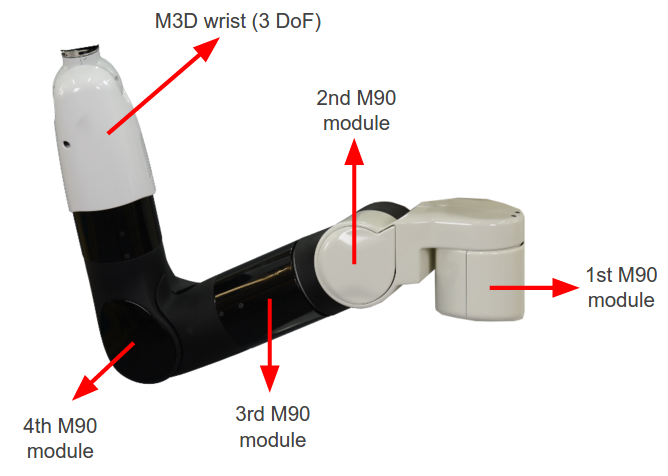
\includegraphics[width=\linewidth]{figures/Arm.png}
    \caption{The 7-DOF arm with its four M90 modules and 3-DOF wrist.
             Image courtesy of PAL Robotics.}
    \label{fig:arm_torso}
  \end{minipage}
  \hfill
  \begin{minipage}{0.48\textwidth}
    \centering
    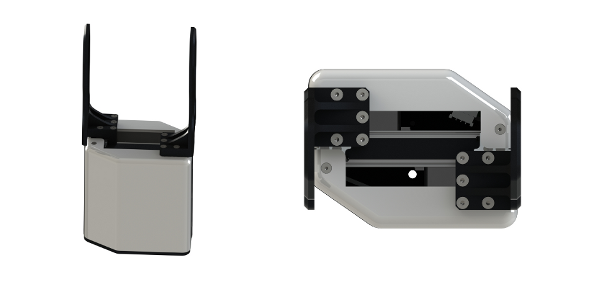
\includegraphics[width=\linewidth]{figures/Parallel_gripper.png}
    \caption{The PAL parallel two-finger gripper.
             Image courtesy of PAL Robotics.}
    \label{fig:gripper_head}
  \end{minipage}
\end{figure}

The robot's \textbf{head} carries the main perception sensor: an \textbf{Asus
Xtion Pro Live} structured-light RGB-D camera that provides registered colour
and depth images at up to 30\,fps at $640\times480$ resolution
(Figure~\ref{fig:head_kinematics}).
The head itself has two degrees of freedom --- pan (horizontal rotation,
$\pm1.5$\,rad) and tilt (vertical angle, $-0.8$ to $+0.4$\,rad) --- which allows
the camera to survey a wide field around the robot during object search.

\begin{figure}[H]
  \centering
  \begin{minipage}{0.48\textwidth}
    \centering
    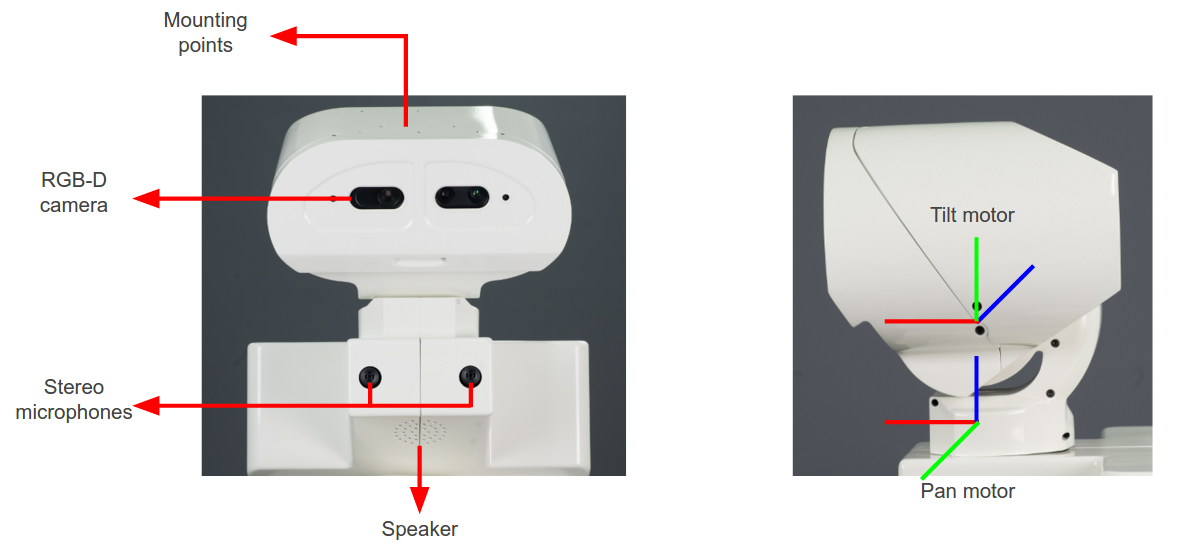
\includegraphics[width=\linewidth]{figures/Head_parts.png}
    \caption{TIAGo head assembly with the Xtion RGB-D camera, stereo microphone,
             and pan-tilt joints. Image courtesy of PAL Robotics.}
    \label{fig:head_kinematics}
  \end{minipage}
  \hfill
  \begin{minipage}{0.48\textwidth}
    \centering
    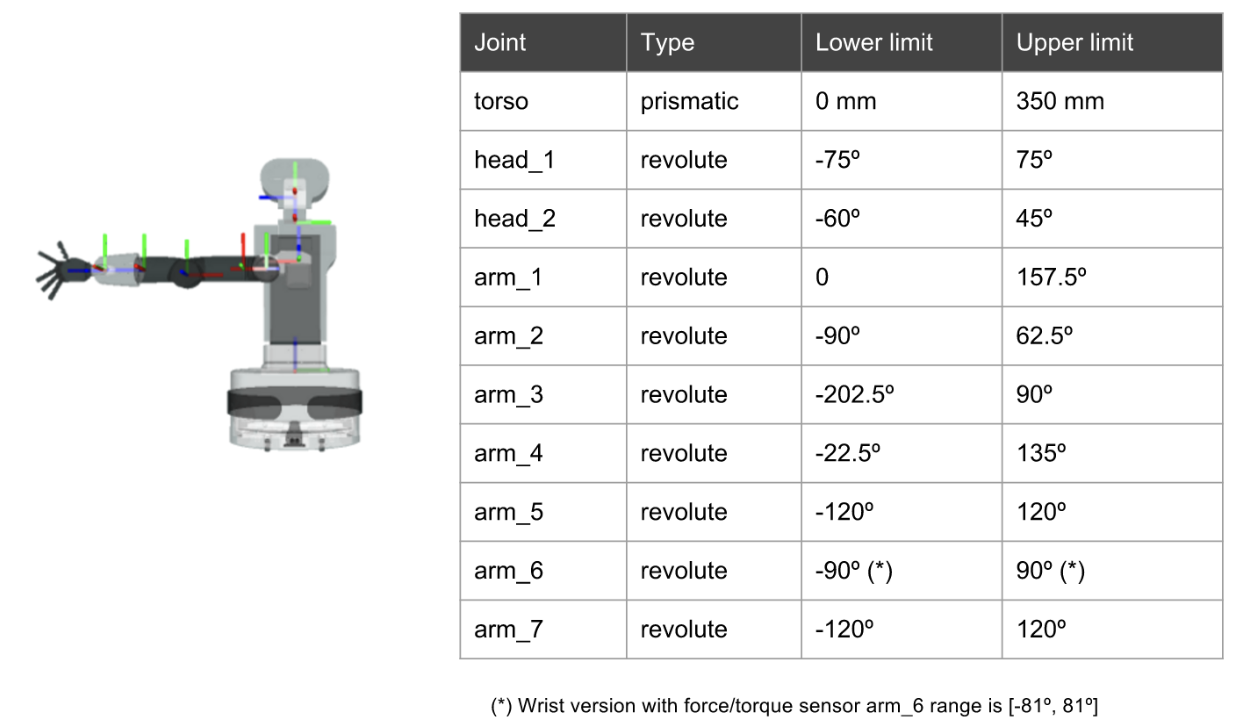
\includegraphics[width=\linewidth]{figures/kinematics.png}
    \caption{Upper-body kinematic structure and joint motion ranges.
             Image courtesy of PAL Robotics.}
    \label{fig:kinematics_detail}
  \end{minipage}
\end{figure}

A critical hardware constraint that shaped the entire software architecture is
that the robot's onboard computer runs \textbf{ROS Melodic under Ubuntu 18.04
inside a Docker container}, limiting the Python runtime to version 3.6.
This is incompatible with modern deep-learning inference frameworks (PyTorch,
ONNX Runtime, Ultralytics), all of which require Python 3.8 or later.
The architectural solution to this constraint is described in the next section.

% ============================================================
\section{Full System Architecture}
\label{sec:architecture}
% ============================================================

The TIAGo VLA agent is structured as a \textbf{four-layer heterogeneous system}
spanning a cloud reasoning service, a host machine running the neural network
inference, a Docker container executing all ROS and agent code, and the physical
robot hardware.
The central organising pattern is the \textbf{perceive-reason-act loop}: at each
cycle the agent captures an annotated image of the scene, sends it to a cloud
VLM that decides what to do next, executes the chosen skill on the robot, and
repeats until the task is complete.
Figure~\ref{fig:arch_full} shows the complete architecture with all components
and communication channels.

\begin{landscape}
\begin{figure}[p]
\centering
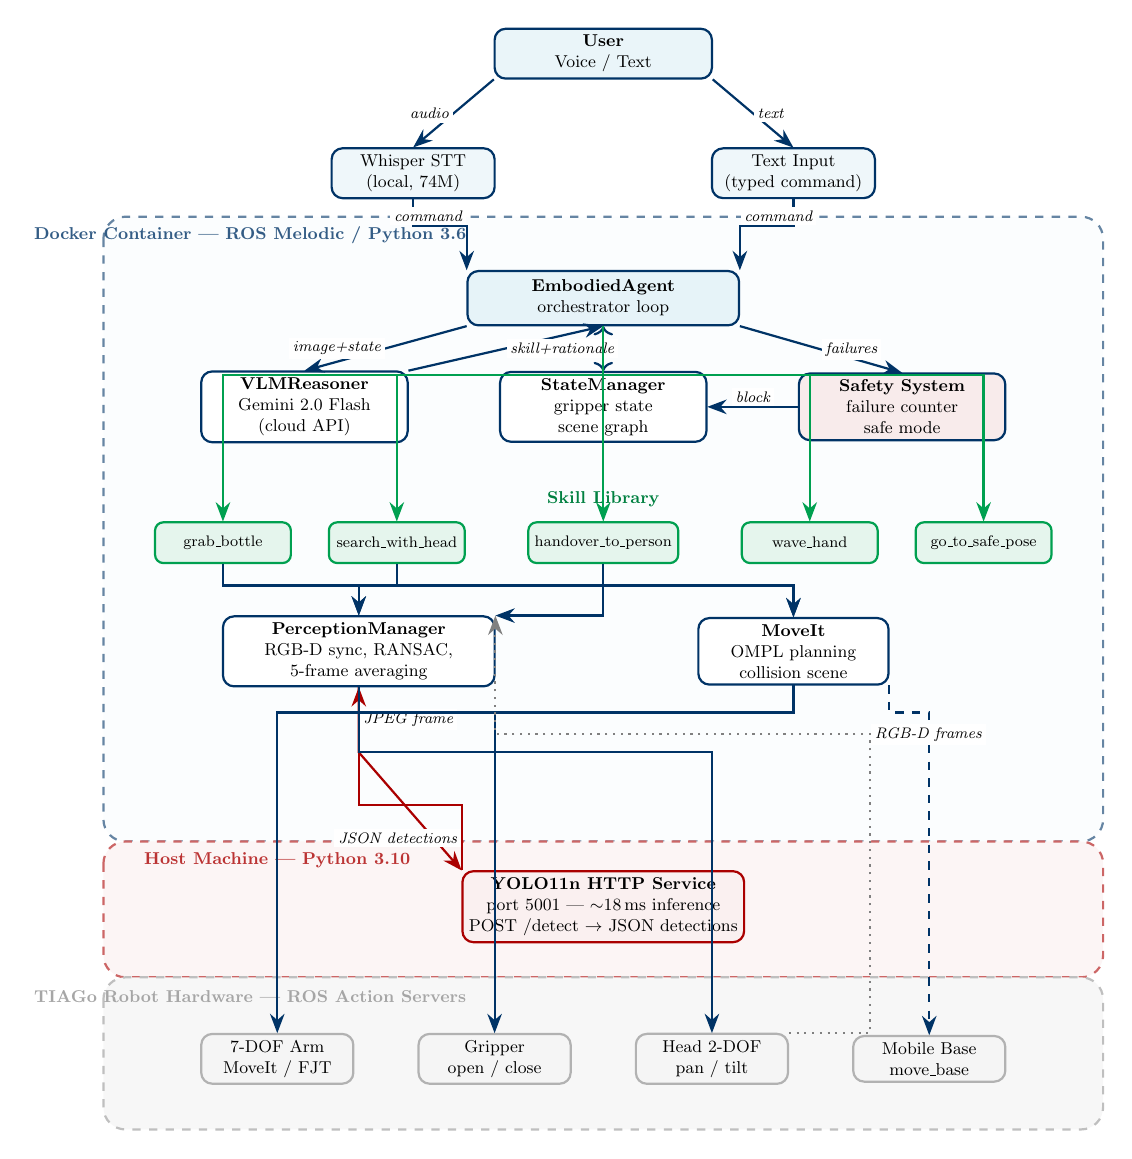
\begin{tikzpicture}[scale=0.69, transform shape,
  %--- node styles ---
  layer/.style={rectangle, rounded corners=6pt, draw=darkblue, very thick,
                minimum width=18cm, minimum height=1.0cm,
                fill=lightblue!12, font=\bfseries\small},
  box/.style={rectangle, rounded corners=4pt, draw=darkblue, thick,
              fill=white, minimum width=3.0cm, minimum height=0.85cm,
              align=center, font=\small},
  skillbox/.style={rectangle, rounded corners=3pt, draw=palgreen, thick,
                   fill=palgreen!10, minimum width=2.5cm, minimum height=0.75cm,
                   align=center, font=\footnotesize},
  hostbox/.style={rectangle, rounded corners=4pt, draw=codered, thick,
                  fill=codered!6, minimum width=4.5cm, minimum height=0.85cm,
                  align=center, font=\small},
  hwbox/.style={rectangle, rounded corners=4pt, draw=gray!60, thick,
                fill=gray!8, minimum width=2.8cm, minimum height=0.8cm,
                align=center, font=\small},
  boundary/.style={rectangle, rounded corners=8pt, dashed, thick},
  arr/.style={-{Stealth[length=7pt]}, thick, draw=darkblue},
  arrg/.style={-{Stealth[length=7pt]}, thick, draw=palgreen},
  arrr/.style={-{Stealth[length=7pt]}, thick, draw=codered},
  lbl/.style={font=\footnotesize\itshape, fill=white, inner sep=2pt},
]

%% ---- ROW 0: User ------------------------------------------
\node[box, fill=lightblue!25, minimum width=4cm] (user) at (0, 0)
  {\textbf{User}\\Voice / Text};

%% ---- ROW 1: Input processing ------------------------------
\node[box, fill=lightblue!20] (stt) at (-3.5, -2.2)
  {Whisper STT\\(local, 74M)};
\node[box, fill=lightblue!20] (txt) at (3.5, -2.2)
  {Text Input\\(typed command)};

%% ---- DOCKER BOUNDARY --------------------------------------
\draw[boundary, fill=lightblue!5, draw=darkblue!60]
  (-9.2, -3.0) rectangle (9.2, -14.5);
\node[font=\small\bfseries, text=darkblue!80] at (-6.5, -3.35)
  {Docker Container --- ROS Melodic / Python 3.6};

%% ---- ROW 2: Agent core ------------------------------------
\node[box, fill=lightblue!30, minimum width=5cm, minimum height=1.0cm]
  (agent) at (0, -4.5) {\textbf{EmbodiedAgent}\\orchestrator loop};

\node[box, minimum width=3.8cm] (vlm) at (-5.5, -6.5)
  {\textbf{VLMReasoner}\\Gemini 2.0 Flash\\(cloud API)};
\node[box, minimum width=3.8cm] (state) at (0, -6.5)
  {\textbf{StateManager}\\gripper state\\scene graph};
\node[box, minimum width=3.8cm, fill=codered!8] (safety) at (5.5, -6.5)
  {\textbf{Safety System}\\failure counter\\safe mode};

%% ---- ROW 3: Skills ----------------------------------------
\node[font=\small\bfseries, text=palgreen!80!black] at (0, -8.2) {Skill Library};
\node[skillbox] (sgrab)   at (-7.0, -9.0) {grab\_bottle};
\node[skillbox] (ssearch) at (-3.8, -9.0) {search\_with\_head};
\node[skillbox] (shand)   at (0.0, -9.0)  {handover\_to\_person};
\node[skillbox] (swave)   at (3.8, -9.0)  {wave\_hand};
\node[skillbox] (spose)   at (7.0, -9.0)  {go\_to\_safe\_pose};

%% ---- ROW 4: Perception ------------------------------------
\node[box, minimum width=5cm] (perc) at (-4.5, -11.0)
  {\textbf{PerceptionManager}\\RGB-D sync, RANSAC,\\5-frame averaging};

\node[box, minimum width=3.5cm] (moveit) at (3.5, -11.0)
  {\textbf{MoveIt}\\OMPL planning\\collision scene};

%% ---- HOST BOUNDARY ----------------------------------------
\draw[boundary, fill=codered!4, draw=codered!60]
  (-9.2, -14.5) rectangle (9.2, -17.0);
\node[font=\small\bfseries, text=codered!80] at (-6.0, -14.85)
  {Host Machine --- Python 3.10};
\node[hostbox] (yolo) at (0, -15.7)
  {\textbf{YOLO11n HTTP Service}\\port 5001 --- $\sim$18\,ms inference\\POST /detect $\rightarrow$ JSON detections};

%% ---- ROBOT HARDWARE  (below host) -------------------------
\draw[boundary, fill=gray!6, draw=gray!50]
  (-9.2, -17.0) rectangle (9.2, -19.8);
\node[font=\small\bfseries, text=gray!70] at (-6.5, -17.35)
  {TIAGo Robot Hardware --- ROS Action Servers};
\node[hwbox] (hw_arm)  at (-6.0, -18.5) {7-DOF Arm\\MoveIt / FJT};
\node[hwbox] (hw_grip) at (-2.0, -18.5) {Gripper\\open / close};
\node[hwbox] (hw_head) at (2.0,  -18.5) {Head 2-DOF\\pan / tilt};
\node[hwbox] (hw_base) at (6.0,  -18.5) {Mobile Base\\move\_base};

%% ---- ARROWS -----------------------------------------------
% User -> STT / Text
\draw[arr] (user.south west) -- node[lbl,left]{audio} (stt.north);
\draw[arr] (user.south east) -- node[lbl,right]{text} (txt.north);
% STT/Text -> Agent
\draw[arr] (stt.south)  -- ++(0,-0.5) -| node[lbl,above left]{command} (agent.north west);
\draw[arr] (txt.south)  -- ++(0,-0.5) -| node[lbl,above right]{command}(agent.north east);
% Agent <-> VLM
\draw[arr] (agent.south west) -- node[lbl,left]{image+state} (vlm.north);
\draw[arr] (vlm.north east)   -- node[lbl,right]{skill+rationale} (agent.south);
% Agent <-> State
\draw[arr,<->] (agent.south) -- (state.north);
% Agent <-> Safety
\draw[arr] (agent.south east) -- node[lbl,right]{failures} (safety.north);
\draw[arr] (safety.west) -- node[lbl,above]{block} (state.east);
% Agent -> Skills
\draw[arrg] (agent.south) -- ++(0,-0.9) -| (sgrab.north);
\draw[arrg] (agent.south) -- ++(0,-0.9) -| (ssearch.north);
\draw[arrg] (agent.south) -- ++(0,-0.9) -- (shand.north);
\draw[arrg] (agent.south) -- ++(0,-0.9) -| (swave.north);
\draw[arrg] (agent.south) -- ++(0,-0.9) -| (spose.north);
% Skills -> Perception
\draw[arr] (sgrab.south)   -- ++(0,-0.4) -| (perc.north);
\draw[arr] (ssearch.south) -- ++(0,-0.4) -| (perc.north);
\draw[arr] (shand.south)   -- ++(0,-0.4) |- (perc.north east);
% Skills -> MoveIt
\draw[arr] (sgrab.south)   -- ++(0,-0.4) -| (moveit.north);
\draw[arr] (shand.south)   -- ++(0,-0.4) -| (moveit.north);
% Perception <-> YOLO
\draw[arrr] (perc.south) -- ++(0,-0.6) node[lbl,right]{JPEG frame}
            -- ++(0,-0.6) -- (yolo.north west);
\draw[arrr] (yolo.north west) -- ++(0,0.6) node[lbl,left]{JSON detections}
            -- ++(0,0.6) -| (perc.south);
% MoveIt -> Arm/Gripper HW
\draw[arr] (moveit.south) -- ++(0,-0.5) -| (hw_arm.north);
\draw[arr] (moveit.south) -- ++(0,-0.5) -| (hw_grip.north);
% Perception -> Head HW
\draw[arr] (perc.south) -- ++(0,-1.2) -| (hw_head.north);
% Perception -> Base
\draw[arr, dashed] (moveit.south east) -- ++(0,-0.5) -| (hw_base.north);
% Camera -> Perception (feedback)
\draw[arr, dotted, draw=gray] (hw_head.north east) -- ++(1.5,0)
  -- ++(0,5.5) node[lbl,right]{RGB-D frames} -| (perc.north east);

\end{tikzpicture}
\caption{Full architecture of the TIAGo VLA agent system. The Docker container
  (blue) runs all ROS and agent code under Python~3.6. The host machine (red)
  runs the YOLO11n detection service under Python~3.10 and communicates via
  HTTP. Solid arrows indicate primary data flow; dashed arrows indicate
  navigation commands; dotted arrows indicate sensor feedback.}
\label{fig:arch_full}
\end{figure}
\end{landscape}

\subsection{Architectural Layers}

The diagram in Figure~\ref{fig:arch_full} is best read from top to bottom as a
layered decomposition of concerns, with the user at the top and the physical
robot hardware at the bottom.

\paragraph{User input layer.}
The user issues commands either by speaking into a microphone or by typing at
the terminal.
Spoken audio is routed through \textbf{Whisper STT} (74\,M parameters, running
locally on the laptop CPU), while typed commands bypass speech recognition
entirely.
Both paths produce a plain-text command string that is passed to the agent.

\paragraph{Docker container (Python 3.6, ROS Melodic).}
The innermost blue boundary encloses every component that depends on ROS.
The \textbf{EmbodiedAgent} is the orchestrator: it holds references to all
subsystems, drives the perceive-reason-act loop, and decides when a task is
complete.
Beneath it, three support modules run concurrently.
The \textbf{VLMReasoner} manages all communication with the Gemini API,
encoding images, maintaining conversation history, and parsing JSON responses.
The \textbf{StateManager} subscribes to ROS sensor topics and maintains a
structured, serialisable summary of the robot's state.
The \textbf{Safety System} tracks consecutive failure counts and enforces
safe-mode entry.
Below these, the \textbf{Skill Library} contains seven specialised skill
modules, each inheriting from a common abstract interface.
Two of those skills (\texttt{grab\_bottle} and \texttt{handover\_to\_person})
delegate perception work to the \textbf{PerceptionManager}, which handles
RANSAC-based 3-D localisation, and delegation of arm motion to
\textbf{MoveIt}, the ROS motion planner.

\paragraph{Host machine (Python 3.10).}
The red boundary encloses the \textbf{YOLO11n HTTP Service} --- the one
component that cannot run inside Docker because Ultralytics requires Python 3.8.
The service wraps the model in a minimal Flask server that accepts JPEG frames
via HTTP POST and returns JSON detection arrays.
It is architecturally decoupled from the ROS stack: it can be restarted,
swapped for a different model, or queried by any external tool without touching
the agent code.

\paragraph{Robot hardware (ROS action servers).}
The grey boundary represents the physical TIAGo hardware, accessible from the
Docker container exclusively through typed ROS interfaces.
The arm, gripper, head, and mobile base each expose ROS action servers
(\path{FollowJointTrajectory} for the arm and head;
\path{/parallel\_gripper\_controller} for the gripper;
\path{move\_base} for navigation).
The PAL \path{play\_motion} and \path{/tts} action servers provide higher-level
primitives (named motion trajectories and text-to-speech output) that are used
by the skill library.

\paragraph{Cloud (Google Gemini API).}
The VLMReasoner communicates outward through the Docker network to
Eden AI's \texttt{api.edenai.run} REST endpoint (which proxies to Gemini 2.0 Flash).
This cloud dependency is the single point that requires an internet connection
at runtime; all other system components run on local hardware.

\subsection{The Split-Process Design}

The separation between the Docker container and the host machine is the most
architecturally unusual aspect of the system.
It was originally forced by the Python 3.6 constraint: the Docker image
provided by PAL Robotics for TIAGo ships with Python 3.6 baked in, and
replacing it would break the ROS Melodic Python bindings.
Modern neural network inference frameworks (PyTorch, Ultralytics YOLO,
ONNX Runtime) all require Python 3.8 or later and refuse to install
under 3.6.

Rather than forking or patching the PAL image --- a fragile approach that would
need to be maintained across ROS updates --- the decision was taken to keep the
constraint and work around it architecturally.
The neural network is deployed on the host, which has a clean Python 3.10
environment, and the two processes communicate over the loopback network via HTTP.
Figure~\ref{fig:split_proc} illustrates the boundary.

\begin{figure}[H]
\centering
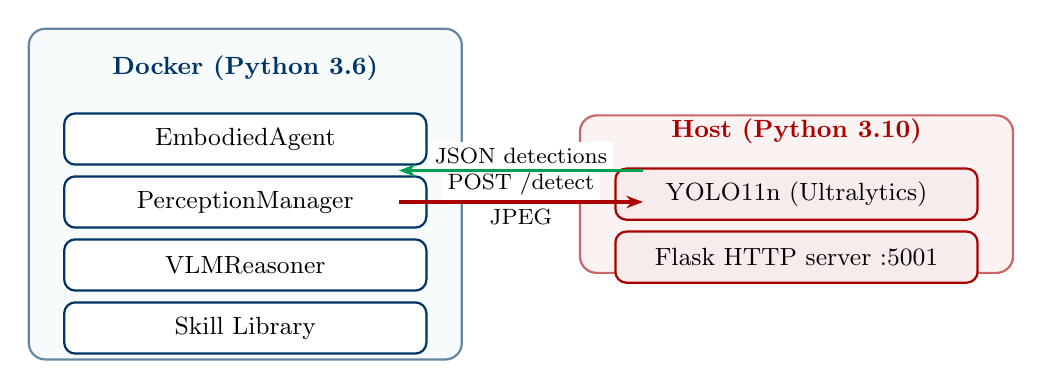
\begin{tikzpicture}[
  proc/.style={rectangle, rounded corners=6pt, draw=darkblue, thick,
               fill=lightblue!15, minimum width=5.5cm, minimum height=3.2cm,
               align=center},
  comp/.style={rectangle, rounded corners=4pt, draw=darkblue, thick,
               fill=white, minimum width=4.6cm, minimum height=0.65cm,
               align=center, font=\small},
  hostcomp/.style={rectangle, rounded corners=4pt, draw=codered, thick,
               fill=codered!8, minimum width=4.6cm, minimum height=0.65cm,
               align=center, font=\small},
  arr/.style={-{Stealth[length=6pt]}, thick},
  lbl/.style={font=\footnotesize, fill=white, inner sep=2pt},
]

% Docker process
\node[proc, draw=darkblue!60, fill=lightblue!10,
      minimum width=5.5cm, minimum height=4.2cm] (docker) at (-3.5,0) {};
\node[font=\small\bfseries, text=darkblue] at (-3.5, 1.6)
  {Docker (Python 3.6)};
\node[comp] at (-3.5,  0.7) {EmbodiedAgent};
\node[comp] at (-3.5, -0.1) {PerceptionManager};
\node[comp] at (-3.5, -0.9) {VLMReasoner};
\node[comp] at (-3.5, -1.7) {Skill Library};

% Host process
\node[proc, draw=codered!60, fill=codered!5,
      minimum width=5.5cm, minimum height=2.0cm] (host) at (3.5,0) {};
\node[font=\small\bfseries, text=codered] at (3.5, 0.8)
  {Host (Python 3.10)};
\node[hostcomp] at (3.5, 0.0) {YOLO11n (Ultralytics)};
\node[hostcomp] at (3.5,-0.8) {Flask HTTP server :5001};

% HTTP arrow
\draw[arr, draw=codered, very thick]
  (-1.55, -0.1) -- node[lbl, above]{POST /detect} node[lbl, below]{JPEG}
  (1.55, -0.1);
\draw[arr, draw=palgreen, very thick]
  (1.55, 0.3) -- node[lbl, above]{JSON detections} (- 1.55, 0.3);

\end{tikzpicture}
\caption{The split-process design: the ROS agent runs in Docker (Python~3.6)
  while the neural network runs on the host (Python~3.10), communicating via
  HTTP on the loopback interface.}
\label{fig:split_proc}
\end{figure}

What began as an unwanted engineering constraint turned out to be a clean
architectural separation.
The concerns are genuinely distinct: the Docker container handles all
real-time robot control (timing-critical ROS callbacks, motion planning,
joint commands), while the host handles GPU-accelerated inference.
Upgrading the detector from YOLO11n to a future model requires only
restarting the microservice on the host; the agent code in Docker is
untouched.
The HTTP interface is also trivially testable: any developer can POST
a JPEG to \texttt{localhost:5001/detect} and inspect the JSON response
without launching ROS.

\subsection{Component Inventory and Interfaces}

Table~\ref{tab:components} lists every software component in the system with
its physical location, programming environment, external interface, and
primary responsibility.

\begin{table}[H]
\centering
\caption{Component inventory: location, interface, and responsibility.}
\label{tab:components}
\small
\begin{tabularx}{\linewidth}{l l X}
\toprule
\textbf{Component} & \textbf{Location / Env.} & \textbf{Interface \& Responsibility} \\
\midrule
EmbodiedAgent      & Docker / Py 3.6  & Central orchestrator; drives perceive-reason-act loop \\
VLMReasoner        & Docker / Py 3.6  & REST POST to Gemini API; returns parsed JSON skill \\
StateManager       & Docker / Py 3.6  & Subscribes \path{/joint_states}, \path{/odom}; exposes \texttt{get\_state()} \\
PerceptionManager  & Docker / Py 3.6  & HTTP client to YOLO service; RANSAC localisation \\
Skill Library (7)  & Docker / Py 3.6  & BaseSkill interface; direct ROS action calls \\
Safety System      & Docker / Py 3.6  & Failure counter; SIGINT/SIGTERM handler \\
MoveIt             & Docker / Py 3.6  & OMPL motion planner; collision scene management \\
YOLO11n Service    & Host / Py 3.10   & Flask HTTP :5001; POST JPEG $\to$ JSON detections \\
Whisper STT        & Host / Py 3.10   & Local speech recognition; 74M Transformer model \\
Gemini 2.0 Flash   & Google Cloud     & REST API; multimodal reasoning, JSON output \\
TIAGo Arm          & Robot HW         & \path{/arm_controller/follow_joint_trajectory} action \\
TIAGo Gripper      & Robot HW         & \path{/parallel_gripper_controller/...} action \\
TIAGo Head         & Robot HW         & \path{/head_controller/follow_joint_trajectory} action \\
play\_motion       & Robot HW         & \path{/play_motion} action; named PAL trajectories \\
PAL TTS            & Robot HW         & \path{/tts} action; text-to-speech in English \\
Mobile Base        & Robot HW         & \path{/move_base} action; 2-D laser navigation \\
\bottomrule
\end{tabularx}
\normalsize
\end{table}

\subsection{Key ROS Topics and Data Flows}

Communication within the Docker container uses standard ROS mechanisms.
Table~\ref{tab:ros_topics} lists the ROS topics that carry sensor data
into the agent and monitoring data out of it.

\begin{table}[H]
\centering
\caption{Key ROS topics used by the agent.}
\label{tab:ros_topics}
\small
\begin{tabularx}{\linewidth}{l l X}
\toprule
\textbf{Topic} & \textbf{Direction} & \textbf{Content} \\
\midrule
\path{/xtion/rgb/image_raw}              & In  & Raw colour frames at 30\,fps ($640\times480$, BGR8) \\
\path{/xtion/depth_registered/image_raw} & In  & Registered depth frames, aligned to RGB frame \\
\path{/xtion/rgb/camera_info}            & In  & Intrinsic calibration: $f_x, f_y, c_x, c_y$ \\
\path{/joint_states}                     & In  & All joint positions including gripper fingers \\
\path{/mobile_base_controller/odom}      & In  & Odometry pose for base-location tracking \\
\path{/agent/camera_annotated}           & Out & Annotated frame with YOLO boxes and depths \\
\path{/agent/status}                     & Out & JSON status: current skill, rationale, state \\
\bottomrule
\end{tabularx}
\normalsize
\end{table}

The \emph{annotated frame} on \path{/agent/camera\_annotated} is the same
image that gets sent to the VLM: YOLO bounding boxes are drawn on the raw
colour frame, with class labels and estimated depths overlaid.
Publishing this on a ROS topic makes it available both to RViz and to the
MJPEG stream on port 8080, so the operator can verify in real time exactly
what the VLM ``sees'' at each reasoning step.
The \path{/agent/status} topic carries a JSON string that is simultaneously
served as a live endpoint on port 8081, enabling the web visualisation
dashboard to display the current skill name, the VLM's stated rationale,
the full state dictionary, and the consecutive failure counter.

% ============================================================
\section{The Perceive-Reason-Act Loop}
\label{sec:loop}
% ============================================================

Every task begins with a command from the user --- either spoken into a USB
microphone or typed at the terminal.
Spoken audio is transcribed locally using \textbf{Whisper base} (74\,M
parameters), a transformer-based speech recognition model that runs in real
time on the laptop CPU and handles accented or lightly imperfect speech
significantly better than classical HMM-based systems.
The agent queries each available audio device in priority order, preferring
the robot's built-in stereo microphone before falling back to any USB audio
device; if no microphone is detected, it falls back to Google Cloud
Speech-to-Text via the \texttt{speech\_recognition} library.

Once the command text is available, the agent opens its \textbf{multi-step
execution loop}, shown in simplified form in Listing~\ref{lst:agent_loop}.
The loop is bounded by two hard limits: a maximum of \texttt{max\_steps = 5}
iterations per task (preventing runaway execution chains) and a
\texttt{max\_consecutive\_failures = 3} threshold that, once exceeded, triggers
a protective safe mode.

\begin{lstlisting}[language=Python, caption={Simplified perceive-reason-act loop in \texttt{EmbodiedAgent.execute\_task()}.}, label={lst:agent_loop}]
def execute_task(self, user_command):
  last_affordance_failure = {}
  last_skill = None

  for step in range(self.max_steps):          # hard limit: 5 steps

    # 1. Capture scene and run detection
    image, detections = self.perception.capture_and_detect()

    # 2. Assemble structured state context
    state = self.state_manager.get_state()

    # 3. Query VLM with image + state + previous failure feedback
    response = self.vlm.query(
      user_command, image, detections, state,
      affordance_failures=last_affordance_failure
    )
    skill_name = response['skill']
    params     = response['parameters']

    # 4. Affordance (precondition) check
    skill    = self.skill_registry[skill_name]
    ok, reason = skill.check_affordance(params, state)
    if not ok:
      last_affordance_failure[skill_name] = reason
      self.consecutive_failures += 1
      if self.consecutive_failures >= self.max_consecutive_failures:
        self._enter_safe_mode()
        return
      continue        # re-query VLM with failure injected

    # 5. Execute skill (blocking)
    last_affordance_failure = {}
    self.consecutive_failures = 0
    skill.execute(params)
    self.state_manager.update(skill_name, success=True)

    # 6. Task completion check
    if response.get('task_complete') or skill_name == last_skill:
      break
    last_skill = skill_name
\end{lstlisting}

\subsection{Affordance Failure Injection}

The most important design detail in the loop is the
\textbf{affordance failure injection} mechanism (lines 14 and 25 of
Listing~\ref{lst:agent_loop}).
When a skill's precondition check fails --- for example, because the VLM
selected \texttt{grab\_bottle} but the gripper is already closed ---
the failure reason string is stored in the \texttt{last\_affordance\_failure}
dictionary, which is passed to the \emph{next} VLM call.
The \texttt{VLMReasoner.query()} method serialises this dictionary and appends
it to the user prompt as a dedicated section:

\begin{mdframed}[style=promptbox]
\texttt{FAILED PRECONDITIONS (do NOT retry these):}\\
\texttt{~~grab\_bottle: gripper already closed ---}\\
\texttt{~~~~~~~~~~~~~~~~choose handover\_to\_person or open\_gripper first}
\end{mdframed}

This closed-loop \emph{inner monologue} feedback --- structurally equivalent to
the Inner Monologue approach of \cite{huang2022inner} --- transforms the VLM
from a brittle one-shot oracle into a self-correcting planner.
Without it, an incorrect VLM decision would simply repeat on the next iteration
and exhaust all allowed steps.
With it, the failure message is injected into the context, and the model
typically corrects itself within one additional iteration.

\subsection{Task Completion Heuristics}

Two complementary conditions terminate the loop.
The primary condition is that the VLM sets \texttt{task\_complete: true} in its
JSON response.
The secondary condition (line 32) encodes a practical heuristic: if the model
selects the same skill on two consecutive steps, the task is considered done.
This catches cases where \texttt{task\_complete} is accidentally omitted after
a successful handover, which would otherwise cause the agent to attempt a second
handover of an already-released object.

% ============================================================
\section{Perception Pipeline}
\label{sec:perception}
% ============================================================

The perception subsystem solves two distinct problems: detecting \emph{what}
objects are in the scene and localising \emph{where} they are in 3-D space.
These are handled by two tightly coupled modules.

\subsection{YOLO11n Object Detection Microservice}

Semantic detection uses \textbf{YOLO11n}, the nano variant of Ultralytics'
latest architecture, running as an HTTP microservice on the host machine's
Python 3.10 environment.
The container sends a raw JPEG frame and receives a JSON array of detections
within approximately 18\,ms --- fast enough for a 15\,fps annotation pipeline.

\begin{lstlisting}[language={}, numbers=none,
    caption={YOLO11n microservice HTTP interface (port 5001).}]
POST http://<HOST_IP>:5001/detect
Content-Type: image/jpeg
X-Classes: bottle,person         # optional server-side class filter

Response (JSON array):
[
  {"class_name": "bottle",  "confidence": 0.87,
   "bbox": [u1, v1, u2, v2]},
  {"class_name": "person",  "confidence": 0.94,
   "bbox": [u1, v1, u2, v2]}
]
\end{lstlisting}

The optional \texttt{X-Classes} header filters detections server-side, which
reduces the JSON payload and avoids exposing irrelevant classes to the VLM.
The service is stateless and restartable independently of the ROS stack, giving
a clean separation of concerns between the AI inference layer and the robot
control layer.

\begin{sloppypar}
YOLO11n was selected over open-vocabulary alternatives
(YOLO-World~\cite{cheng2024yoloworld}, OwlViT~\cite{minderer2022owlvit},
Grounding DINO~\cite{liu2023gdino}) after empirical benchmarking on the
deployment hardware showed that those models required 150--500\,ms per frame
on CPU --- prohibitive for real-time robot control.
The trade-off is that YOLO11n is limited to the 80 COCO classes, but this
covers all objects the agent is currently expected to manipulate (bottles,
cups, bowls, persons).
Table~\ref{tab:yolo_micro} summarises the models evaluated.
\end{sloppypar}

\begin{table}[H]
\centering
\caption{Object detection models evaluated for this deployment.}
\label{tab:yolo_micro}
\small
\begin{tabular}{llll}
\toprule
\textbf{Model} & \textbf{Runtime} & \textbf{CPU infer.} & \textbf{Decision} \\
\midrule
YOLOv4-tiny   & Docker (cv2.dnn)  & $\sim$50\,ms  & Early versions \\
YOLO-World    & Host Py 3.10     & $\sim$150\,ms & Too slow \\
YOLOE-26s-seg & Host Py 3.10     & $\sim$300\,ms & Too slow \\
YOLO11n       & Host microservice & $\sim$18\,ms  & \textbf{Chosen} \\
\bottomrule
\end{tabular}
\normalsize
\end{table}

\subsection{3-D Object Localisation via RANSAC Cylinder Fitting}

Knowing that a bottle exists at pixel coordinates is not sufficient for
grasping --- the arm needs a 3-D position in the robot's base frame.
The localisation pipeline begins by back-projecting the YOLO bounding box onto
the registered depth image from the Xtion sensor.
For each pixel $(u, v)$ inside the bounding box with a valid depth value $d$,
the corresponding 3-D point in camera coordinates is:
\begin{equation}
  \mathbf{p}_{\text{cam}} =
  \begin{pmatrix}
    \dfrac{(u - c_x)\,d}{f_x} \\[6pt]
    \dfrac{(v - c_y)\,d}{f_y} \\[6pt]
    d
  \end{pmatrix}
\end{equation}
where $(f_x, f_y, c_x, c_y)$ are the camera intrinsics read from the
\path{/xtion/rgb/camera_info} topic.

This yields a 3-D point cloud of the object's visible surface.
Rather than taking the raw centroid (which is biased towards the object's
widest face), we fit a cylinder to the cloud in the $XY$ plane using
\textbf{RANSAC}~\cite{schnabel2007ransac}, as formalised in
Algorithm~\ref{alg:ransac}.

\begin{algorithm}[H]
\caption{RANSAC cylinder fitting for 3-D object localisation}
\label{alg:ransac}
\DontPrintSemicolon
\KwIn{Point cloud $\mathcal{P} = \{(x_i, y_i, z_i)\}$; $N_{\text{iter}} = 300$; threshold $\tau = 0.015$\,m; radius range $[r_{\min}, r_{\max}] = [0.015, 0.06]$\,m; $N_{\min\text{pts}} = 15$; $N_{\min\text{inl}} = 8$}
\KwOut{Best cylinder centre $(\hat{x}, \hat{y})$, radius $\hat{r}$; object top $\hat{z}$}
\If{$|\mathcal{P}| < N_{\min\text{pts}}$}{
  \Return{failure: insufficient depth coverage}\;
}
$\text{best\_inliers} \gets \emptyset$\;
\For{$i \gets 1$ \KwTo $N_{\text{iter}}$}{
  Sample 3 random points $\{p_1, p_2, p_3\} \subset \mathcal{P}$\;
  Fit circle $(x_c, y_c, r)$ to $XY$ projections of $\{p_1, p_2, p_3\}$\;
  \If{$r \notin [r_{\min}, r_{\max}]$}{\textbf{continue}\;}
  $\mathcal{I}_i \gets \{p \in \mathcal{P} : \bigl|\sqrt{(p_x-x_c)^2+(p_y-y_c)^2} - r\bigr| < \tau\}$\;
  \If{$|\mathcal{I}_i| > |\text{best\_inliers}|$}{
    $\text{best\_inliers} \gets \mathcal{I}_i$\;
  }
}
\If{$|\text{best\_inliers}| < N_{\min\text{inl}}$}{
  \Return{failure: too few inliers}\;
}
Refine $(\hat{x}, \hat{y}, \hat{r})$ by algebraic least-squares on
$\text{best\_inliers}$ (minimise $\sum_i (\sqrt{\Delta x_i^2+\Delta y_i^2} - r)^2$)\;
$\hat{z} \gets \min\{p_z : p \in \mathcal{P},\; p_v < v_{\min} + \tfrac{1}{4}(v_{\max}-v_{\min})\}$\quad (object top)\;
\Return{$(\hat{x}, \hat{y}, \hat{z})$, $\hat{r}$, inlier\_ratio $= |\text{best\_inliers}|/|\mathcal{P}|$}
\end{algorithm}

After each successful RANSAC fit, a \textbf{frame quality check} is applied:
if the inlier ratio falls below 0.30, the frame is discarded as unreliable.
To further suppress single-frame depth jitter from the Xtion's structured-light
pattern, the 3-D estimate is averaged over \textbf{five consecutive
high-quality frames}:
\begin{equation}
  (\hat{x},\hat{y},\hat{z}) =
  \frac{1}{5}\sum_{i=1}^{5}(x^{(i)},y^{(i)},z^{(i)})
\end{equation}
In practice this reduces the dominant positioning error from
$\sim$15\,mm (single frame) to below 5\,mm for a stationary object ---
well within the tolerance required for the gripper to close around a 500\,ml
bottle.

\subsection{Coordinate-Frame Management under Python 3.6}

A subtle implementation constraint is that the \texttt{tf2\_ros} Python
bindings require Python~3.8 or later; they are unavailable inside the
Docker container.
The solution is to obtain the camera-to-base transform once per grasp attempt
by spawning a subprocess:

\begin{lstlisting}[language=Python, numbers=none]
result = subprocess.check_output(
  ['rosrun', 'tf', 'tf_echo',
   'base_footprint', 'xtion_rgb_optical_frame'],
  timeout=5
)
# Parse translation + quaternion with regex
\end{lstlisting}

The output is parsed with a regular expression to extract the translation
vector and rotation quaternion.
This approach adds approximately 120\,ms per grasp attempt --- negligible
compared with the several seconds required for arm motion --- and has the
advantage of working without any native Python bindings.

% ============================================================
\section{Vision-Language Reasoning}
\label{sec:vlm}
% ============================================================

The VLM is the cognitive centre of the system: it observes an image and the
current context, then decides which action to take next.
This section describes all aspects of the VLM integration, from the API
communication layer to prompt design and failure handling.

\subsection{Model Selection and API Integration}

We chose \textbf{Google Gemini 2.0 Flash} after comparing it with GPT-4o and
locally-hosted LLaVA~1.6 on three criteria: inference latency (each agent step
blocks on the API response), instruction-following reliability (the model must
always produce valid JSON), and cost (the agent may invoke the VLM five or more
times per task).
Gemini 2.0 Flash consistently produced valid JSON on the first attempt,
responded in 1--4\,s, and cost approximately \$0.005 per call --- significantly
cheaper per image than GPT-4o.

The model is accessed via the \textbf{Generative Language REST API} rather than
the Python SDK (which requires Python~3.8):

\begin{lstlisting}[language={}, numbers=none,
    caption={REST API endpoint for Gemini 2.0 Flash via Eden AI.}]
POST https://api.edenai.run/v3/llm/chat/completions
Authorization: Bearer <EDENAI_API_KEY>
Content-Type: application/json
Body: {"model": "google/gemini-2-0-flash", "messages": [...], "max_tokens": 300}
\end{lstlisting}

The \texttt{VLMReasoner} class implements 3 automatic retries with exponential
back-off on HTTP errors.
If all retries fail or the response cannot be parsed as valid JSON (after
stripping any markdown code fences the model may accidentally include), the
reasoner returns a safe fallback: \texttt{\{"skill": "go\_to\_safe\_pose", ...
\}}.
This ensures that a transient network failure degrades gracefully to a safe arm
pose rather than an uncontrolled state.

\subsection{Image Encoding and Cost Optimisation}

Sending raw camera frames to the API would be both slow and expensive.
Before encoding, each image is resized so that its longest dimension does not
exceed \textbf{640 pixels} and re-compressed at \textbf{JPEG quality 85}:

\begin{lstlisting}[language=Python, numbers=none]
def encode_image(pil_image, max_size=640, quality=85):
  w, h = pil_image.size
  if max(w, h) > max_size:
    scale = max_size / max(w, h)
    pil_image = pil_image.resize(
      (int(w*scale), int(h*scale)), Image.LANCZOS)
  buffer = io.BytesIO()
  pil_image.save(buffer, format='JPEG', quality=quality)
  return base64.b64encode(buffer.getvalue()).decode('utf-8')
\end{lstlisting}

This reduces the per-image payload from $\sim$900\,KB (raw $640\times480$ RGB)
to approximately 35--50\,KB, cutting API transfer cost and latency without
meaningfully degrading the model's visual understanding for manipulation
tasks.

\subsection{Prompt Design}

The system prompt is the most important single engineering artefact in the
project: it defines the model's persona, its available actions, its output
contract, and the behavioural rules that prevent common failure modes.

\begin{mdframed}[style=promptbox]
\small
\textbf{SYSTEM PROMPT (condensed)}\\[4pt]
You are the cognitive controller of TIAGo, a PAL Robotics mobile manipulator.
Your role: observe the camera image, analyse the scene, and select the next
skill to execute.\\[4pt]
\textbf{Available skills:}\\
\texttt{grab\_bottle} | \texttt{search\_with\_head} |
\texttt{handover\_to\_person}\\
\texttt{wave\_hand} | \texttt{open\_gripper} | \texttt{close\_gripper} |
\texttt{go\_to\_safe\_pose}\\[4pt]
\textbf{Current state injected here:}\\
\texttt{gripper: open | base\_location: table}\\
\texttt{detected: [bottle @(0.3m, 0.1m), person @(1.5m)]}\\
\texttt{history: [grab\_bottle(success), ...]}\\[4pt]
\textbf{Output --- respond ONLY with valid JSON, no markdown, no prose:}\\
\texttt{\{"skill": "...", "parameters": \{...\}, "rationale": "...",}\\
\texttt{~"task\_complete": false\}}\\[4pt]
\textbf{Rules:} Never retry a skill listed in FAILED PRECONDITIONS.
Search before grasping an invisible object. If gripper is already closed,
do not attempt another grasp. Set \texttt{task\_complete: true} when done.
Express reasoning in \texttt{rationale} before choosing an action.
\end{mdframed}

The strict output constraint (\emph{``Respond ONLY with valid JSON, no
markdown, no prose''}) was essential.
Early iterations without this constraint produced free-text replies that
required fragile regex parsing and failed roughly 20\% of the time.
The current design reduces parse failures to negligible levels.

\subsection{Conversation History and Rolling Context}

The VLMReasoner maintains a \textbf{rolling 20-turn dialogue history}
(10 user + 10 model turns).
This history is included verbatim in every API call, giving the model
persistent memory of the task's progress: which skills executed successfully,
which objects were detected in previous frames, and which preconditions
previously failed.
When the history reaches 20 turns, the oldest pair is dropped in a FIFO
fashion to keep the context within the API's token limit.

\subsection{Post-Execution Verification}

After each skill execution, an optional \textbf{visual verification} step
sends two images --- a ``before'' snapshot captured just before the skill
and an ``after'' snapshot captured immediately after --- to the VLM with
a verification prompt.
The model returns a JSON object:
\begin{lstlisting}[language=JSON, numbers=none]
{"success": true,
 "observation": "Gripper closed around bottle, arm raised.",
 "issue": null}
\end{lstlisting}

This verification step is not on the critical execution path (failures do not
abort the task) but is logged for analysis and surfaced in the live
visualisation dashboard.

% ============================================================
\section{Manipulation and Grasping}
\label{sec:manipulation}
% ============================================================

Grasping is the most mechanically demanding capability in the system and the
part that required the most iterative development.
The final pipeline (version 5) went through five distinct design revisions,
each addressing a specific failure mode found during real-robot testing.

\subsection{From v1 to v5: An Iterative Journey}

\textbf{Version 1} used a simple MoveIt Cartesian goal directly in the robot's
base frame, relying on YOLO bounding-box centroids for the 3-D position.
It produced a working prototype, but single-frame depth noise caused the arm
to miss the object by 2--4\,cm, and the gripper had no calibrated offset
relative to the arm tool link.

\textbf{Version 2} addressed noise by introducing 5-frame temporal averaging
of depth estimates and added proper frame alignment between camera and base
using ROS TF.
This halved positioning errors but still relied on raw point-cloud centroids.

\textbf{Version 3} integrated the PAL parallel gripper with hand-calibrated
mechanical offsets measured using an interactive calibration script
(\texttt{calibrate\_grasp\_interactive.py}).
This brought the gripper reliably above the object centre, but Cartesian IK
failures near the table surface limited robustness.

\textbf{Version 4} replaced bounding-box centroids with RANSAC cylinder
fitting, exploiting the object's geometry for a more accurate and robust
centre estimate.
This dramatically improved accuracy for thin cylindrical objects (bottles)
and reduced false grasp attempts caused by centroid bias.

\textbf{Version 5} addressed the remaining IK failures by replacing the
Cartesian final-approach path with the \textbf{torso-descent} vertical
approach described below.

\subsection{The v5 Grasping Pipeline}

The complete v5 grasp sequence is as follows.

\begin{enumerate}[noitemsep]
  \item \textbf{Orient head.}
        Tilt the head to $-0.5$\,rad (looking down at the table), reading the
        current pan angle from \path{head_1_joint} on \path{/joint_states}
        to preserve the lateral direction already pointing at the object.

  \item \textbf{Unfold arm.}
        Command \texttt{play\_motion(``pregrasp\_bottle'')} to move the arm
        from its tucked rest configuration to a ready pose that clears
        the torso and base.

  \item \textbf{Open gripper.}
        Issue an open command via the gripper action server.

  \item \textbf{Record TF transform.}
        Obtain the camera-to-base transform once via \texttt{rosrun tf
        tf\_echo} (Section~\ref{sec:perception}).

  \item \textbf{Run 5-frame RANSAC localisation.}
        Collect five consecutive high-quality RANSAC fits and average them
        to obtain $(\hat{x}, \hat{y}, \hat{z})$ in the base frame.

  \item \textbf{Build collision scene.}
        Add two collision objects to MoveIt: a table box
        ($0.8\times1.2\times0.02$\,m centred 1\,cm below the estimated
        surface) and a cylindrical object placeholder with radius
        $(\hat{r} + 0.01)$\,m.

  \item \textbf{Move arm above object.}
        Command MoveIt with a \texttt{PoseStamped} goal positioned
        \texttt{descent = 0.20}\,m above the estimated grasp height,
        with the gripper oriented downward.

  \item \textbf{Torso descent.}
        Lower the torso joint from its current position to bring the
        gripper exactly to the grasp height.
        Because the torso is a world-Z-aligned prismatic joint, this
        guarantees a straight vertical trajectory with no IK computation.

  \item \textbf{Close gripper and lift.}
        Close the gripper with a maximum current limit of
        \textbf{0.35\,A} (preventing damage to soft objects), then raise
        the torso to lift the object 5\,cm off the table surface.
\end{enumerate}

\subsection{Calibrated Grasp Parameters}

The pre-grasp goal pose is expressed relative to the RANSAC-estimated object
centre using empirically calibrated offsets measured during development.
Table~\ref{tab:grasp_params} lists the final calibrated values.

\begin{table}[H]
\centering
\caption{Empirically calibrated v5 grasp parameters.}
\label{tab:grasp_params}
\small
\begin{tabularx}{\linewidth}{l p{3.8cm} X}
\toprule
\textbf{Parameter} & \textbf{Value} & \textbf{Description} \\
\midrule
Forward offset $\Delta x$    & $0.19$\,m    & Gripper to object centre along base-X \\
Lateral offset $\Delta y$    & $0.05$\,m    & Correction for gripper-to-tool-link asymmetry \\
Vertical offset $\Delta z$   & $0.0361$\,m  & Height of gripper fingers above object top \\
Descent distance             & $0.20$\,m    & Torso travel for final vertical approach \\
Gripper orient.\ $q$         & $(-0.640,\,-0.080,$\newline$\phantom{(}-0.020,\,+0.764)$ & Quaternion $(x,y,z,w)$ for downward grasp \\
Max gripper current          & $0.35$\,A    & Current limit to protect soft objects \\
\bottomrule
\end{tabularx}
\normalsize
\end{table}

The orientation quaternion $(-0.640,\,-0.080,\,-0.020,\,+0.764)$ was determined
by commanding the arm to the desired downward-pointing pose in MoveIt's
interactive marker, reading back the wrist joint quaternion, and hard-coding it.
Small deviations from perfect vertical ($x=-1,\,y=z=0,\,w=0$) in the
$y$- and $z$-components reflect the mechanical asymmetry of the PAL gripper
attachment and were retained as measured.

\subsection{Visual Search: The 12-Position Head Sweep}

When the VLM selects \texttt{search\_with\_head} because the target object is
not visible, the robot executes a systematic head sweep across twelve pan/tilt
positions that cover the full reachable field of view around the robot's
current position.
At each position, the head settles for 2\,s (allowing the image to stabilise)
before querying the YOLO service.
The sweep terminates as soon as the target class is detected with
confidence $>$\,0.4, or returns failure if all twelve positions have been
scanned without a detection.
Table~\ref{tab:search_positions} lists the twelve positions in scan order.

\begin{table}[H]
\centering
\caption{Head sweep positions for \texttt{search\_with\_head} skill (12 positions in order).}
\label{tab:search_positions}
\small
\begin{tabular}{clrrp{4.5cm}}
\toprule
\textbf{\#} & \textbf{Name} & \textbf{Pan (rad)} & \textbf{Tilt (rad)} & \textbf{Field covered} \\
\midrule
1  & centre          &  0.0  &  0.00  & Straight ahead, horizontal \\
2  & centre\_down    &  0.0  & $-0.45$  & Straight ahead, looking down \\
3  & left            &  0.8  &  0.00  & Left quarter \\
4  & left\_down      &  0.8  & $-0.45$  & Left quarter, looking down \\
5  & far\_left       &  1.4  &  0.00  & Hard left \\
6  & far\_left\_down &  1.4  & $-0.45$  & Hard left, looking down \\
7  & right           & $-0.8$  &  0.00  & Right quarter \\
8  & right\_down     & $-0.8$  & $-0.45$  & Right quarter, looking down \\
9  & far\_right      & $-1.4$  &  0.00  & Hard right \\
10 & far\_right\_down & $-1.4$ & $-0.45$ & Hard right, looking down \\
11 & up              &  0.0  & $+0.30$ & Straight ahead, elevated \\
12 & centre (return) &  0.0  &  0.00  & Reset to forward gaze \\
\bottomrule
\end{tabular}
\normalsize
\end{table}

A key implementation detail is that the tilt command reads the current pan
value from \path{/joint_states} before issuing the new head goal.
This prevents the head from snapping to the centre pan on every tilt change,
which would miss objects to the side and produce jerky motion.

\subsection{Person Handover Skill}

The \texttt{handover\_to\_person} skill completes the full
``find -- grasp -- deliver'' task chain.
Its affordance condition requires that the gripper is closed (holding an object)
\emph{and} that a person class detection is present in the current frame.

The execution sequence is:

\begin{enumerate}[noitemsep]
  \item \textbf{Detect person region.}
        Extract the YOLO bounding box for the nearest ``person'' detection.
        The person's estimated body centre is taken as the midpoint of the
        bounding box's middle horizontal and lower-vertical thirds.

  \item \textbf{Estimate person depth.}
        Back-project the body-centre pixel through the Xtion depth image
        to obtain the person's approximate 3-D position in the base frame.

  \item \textbf{Clear the octomap.}
        Call the \path{/clear_octomap} service to remove stale voxels
        around the person's position so that MoveIt can plan a
        collision-free path to the handover pose.

  \item \textbf{Add person collision box.}
        Insert a $0.50 \times 0.50 \times 1.80$\,m box at the estimated
        person position in the MoveIt planning scene.
        This prevents the arm from swinging through the person during
        trajectory planning.

  \item \textbf{Plan and execute arm motion.}
        Command MoveIt to a handover pose at:
        \[
          \text{height} = \text{HANDOVER\_HEIGHT} = 0.85\,\text{m},
          \quad
          \text{reach} = \text{ARM\_REACH} = 0.62\,\text{m}
        \]
        oriented toward the estimated person direction.

  \item \textbf{Wait and release.}
        Announce ``\emph{Here you go!}'' via the PAL TTS action server,
        wait 4\,s for the person to take the object, then open the gripper.

  \item \textbf{Clean up.}
        Remove the person collision object from the planning scene and
        return the arm to the pre-grasp pose.
\end{enumerate}

The 4-second wait is intentional: releasing too early (before the person has
grasped the object) would drop it, while waiting indefinitely would stall
the loop.
In practice, 4\,s is sufficient for a person standing within reach to close
their hand around the object.

% ============================================================
\section{Agent Orchestration and Skill Library}
\label{sec:agent}
% ============================================================

The agent is implemented as a class (\texttt{EmbodiedAgent}) that holds
references to all subsystems: the perception manager, the VLM reasoner, the
state manager, and the skill registry.
At initialisation it connects to all ROS action servers, verifies that the
YOLO microservice is reachable, and loads the skill library.
If any critical component is unavailable the agent reports the problem and
exits rather than operating in a degraded mode.

\subsection{Skill Library Design}

Every skill inherits from an abstract \texttt{BaseSkill} class that enforces
a three-method interface:

\begin{lstlisting}[language=Python, numbers=none,
    caption={Abstract base class for all skills.}]
class BaseSkill(ABC):
  @abstractmethod
  def check_affordance(self, params, state) -> Tuple[bool, str]:
    """Return (True, '') if executable, (False, reason) if not."""

  @abstractmethod
  def execute(self, params) -> bool:
    """Execute the skill; return True on success."""

  @abstractmethod
  def get_description(self) -> str:
    """One-line human-readable description for the VLM prompt."""
\end{lstlisting}

This design means that adding a new skill requires only implementing three
methods; the agent loop, precondition checking, failure injection, and
state updates are all handled centrally.

Table~\ref{tab:skill_library} lists the nine skills in the current library
with their affordance conditions.

\begin{table}[H]
\centering
\caption{Skill library: names, preconditions, and actions.}
\label{tab:skill_library}
\begin{tabularx}{\linewidth}{lXX}
\toprule
\textbf{Skill} & \textbf{Precondition} & \textbf{Action} \\
\midrule
\texttt{grab\_bottle}       & Gripper open; bottle visible in frame
                             & v5 nine-step grasp pipeline \\
\texttt{search\_with\_head} & None (always executable)
                             & 12-position pan/tilt sweep \\
\texttt{handover\_to\_person} & Gripper closed; person visible in frame
                             & Arm reach to 0.85\,m, open gripper \\
\texttt{wave\_hand}         & None
                             & play\_motion(``wave'') trajectory \\
\texttt{open\_gripper}      & Gripper closed
                             & Open gripper action \\
\texttt{close\_gripper}     & Gripper open
                             & Close gripper action \\
\texttt{go\_to\_safe\_pose} & None
                             & Tuck arm, open gripper \\
\bottomrule
\end{tabularx}
\end{table}

\subsection{State Manager}

The \texttt{StateManager} provides the VLM with a structured, persistent view
of the robot's state between loop iterations.
It subscribes to two ROS topics:

\begin{sloppypar}
\begin{itemize}
  \item \path{/joint_states} --- to infer gripper state from the
        \texttt{parallel\_gripper\_right\_finger\_joint} position:
        below 0.005\,m the gripper is treated as \emph{open};
        above 0.015\,m it is \emph{closed}.
        Values in between indicate a transition in progress.

  \item \path{/mobile_base_controller/odom} --- to track the robot's
        approximate base location for context-aware skill selection.
\end{itemize}
\end{sloppypar}

On each call to \texttt{get\_state()}, the manager returns a dictionary
containing:
(1) the current gripper state,
(2) the estimated base location,
(3) the most recent five detected objects with their pixel bounding boxes,
(4) the last three entries of the task history in the form
    ``\texttt{[+] grab\_bottle}'' / ``\texttt{[-] grab\_bottle}'', and
(5) up to ten spatial relations inferred from the detection geometry.

\paragraph{Scene graph inference.}
Spatial relations are inferred from the pixel positions of YOLO detections.
Two objects are marked as \emph{near} if the distance between their bounding-box
centres is below 150\,px.
Objects whose centres lie within 50\,px vertically are inferred as being
\emph{on the same surface}, which the state manager reports as ``on table''
when all such objects are at a consistent height.
Left/right and above/below relations are added for all object pairs whose
bounding boxes do not overlap.
This gives the VLM a lightweight semantic scene description without requiring
an explicit 3-D map.

\subsection{Live Visualisation}

To facilitate debugging and demonstrations, the agent publishes two continuous
output streams.
The \textbf{annotated image} --- the same frame sent to Gemini, with bounding
boxes and estimated depths overlaid --- is published on
\path{/agent/camera_annotated} (ROS \texttt{sensor\_msgs/Image}, BGR8) and
streamed as MJPEG on port 8080.
A \textbf{JSON status packet} containing the current skill name, VLM rationale,
full state dictionary, and consecutive failure count is published on
\path{/agent/status} (ROS \texttt{std\_msgs/String}) and served as a live
JSON endpoint on port 8081.
Both streams are accessible in a standard web browser without installing any
additional software.

% ============================================================
\section{Safety Architecture}
\label{sec:safety}
% ============================================================

Safety was designed in from the start rather than added as an afterthought.
The system has three complementary layers: affordance gating (preventing
physically unsafe actions before they start), failure counting (detecting
repeated failures), and graceful shutdown (recovering to a known safe state
in response to any termination signal).

\subsection{Affordance Gating}

Every skill exposes a \texttt{check\_affordance} method that the agent calls
\emph{before} sending any motion command to the robot.
If the precondition returns false, the skill is not executed; instead, the
failure reason is injected into the next VLM prompt via the affordance failure
mechanism described in Section~\ref{sec:loop}.
This layer prevented several potentially damaging arm movements during early
development, including cases where the VLM attempted a second grasp with the
gripper already loaded with a bottle.

\subsection{Consecutive Failure Counting and Safe Mode}

\begin{sloppypar}
The agent tracks the number of consecutive affordance or execution failures
in a counter that resets to zero on any successful skill completion.
When the counter reaches \texttt{max\_consecutive\_failures}$\,=3$, the agent
calls \texttt{\_enter\_safe\_mode()}:
\end{sloppypar}

\begin{enumerate}[noitemsep]
  \item Set the \texttt{safe\_mode} flag to \texttt{True} (blocks all further
        skill dispatch).
  \item Execute \texttt{go\_to\_safe\_pose} unconditionally.
  \item Announce the failure via TTS: \emph{``I am having trouble. Please check
        my state.''}.
  \item Wait for an operator \texttt{reset} command before resuming.
\end{enumerate}

\subsection{Graceful Shutdown on Interrupt}

The agent registers handlers for both \texttt{SIGINT} (keyboard interrupt) and
\texttt{SIGTERM} (system termination) that call a
\texttt{\_safe\_shutdown()} method before exiting:

\begin{lstlisting}[language=Python, numbers=none,
    caption={Signal handler for safe shutdown.}]
def _safe_shutdown(self):
  try:
    self.skills['open_gripper'].execute({})    # release held object
    self.skills['go_to_safe_pose'].execute({}) # tuck arm
  finally:
    rospy.signal_shutdown('Agent terminated')
  sys.exit(0)
\end{lstlisting}

This ensures that the robot always ends in a safe, tucked pose regardless
of how the agent is stopped --- whether by the operator pressing Ctrl-C,
a deployment script sending SIGTERM, or a Python exception that propagates
to the top level.
In practice, this prevented the arm from being left in an extended position
(a significant hazard for nearby persons) on several occasions during
development.

% ============================================================
%  CHAPTER 10 — Experiments and Results
% ============================================================
\chapter{Experiments and Results}
\label{ch:experiments}

\section{Experimental Setup}

All experiments were conducted in a laboratory environment using a single PAL Robotics
\tiago{} robot.
The robot was placed at a fixed position facing a table at approximately 0.8 m distance.
Objects were placed on the table within the camera's field of view and within the
arm's reachable workspace ($\leq$ 0.7 m from the base footprint).

\begin{table}[H]
\centering
\caption{Experimental environment parameters.}
\label{tab:exp_setup}
\begin{tabular}{ll}
\toprule
\textbf{Parameter} & \textbf{Value} \\
\midrule
Table height               & $\approx$ 0.75 m \\
Robot distance to table    & $\approx$ 0.80 m \\
Lighting conditions        & Indoor, artificial \\
Object types tested        & Plastic bottle (500 ml), cup \\
YOLO confidence threshold  & 0.4 \\
Grasp attempts per position& 3 \\
VLM model                  & Gemini 2.0 Flash \\
\bottomrule
\end{tabular}
\end{table}

\section{Experiment 1: YOLO Detection Performance}

\subsection{Inference Speed}

Detection speed was measured by sending the same test image to each model
50 times and recording the mean and standard deviation of inference time.

\begin{table}[H]
\centering
\caption{YOLO inference speed comparison (CPU, 640×480 JPEG input).}
\label{tab:yolo_speed}
\begin{tabular}{lrrrr}
\toprule
\textbf{Model} & \textbf{Mean (ms)} & \textbf{Std (ms)} & \textbf{FPS} & \textbf{Location} \\
\midrule
YOLOv4-tiny (cv2.dnn)  & \todo{XX} & \todo{X} & \todo{XX} & Docker \\
YOLO11n (service)      & \todo{XX} & \todo{X} & \todo{XX} & Host \\
YOLOE-26s-seg          & \todo{XX} & \todo{X} & \todo{XX}  & Host \\
\bottomrule
\end{tabular}
\end{table}

\subsection{Detection Quality}

A set of 30 images of a bottle at varying distances, angles, and lighting conditions
was prepared.
YOLO11n was evaluated on these images with a confidence threshold of 0.4.

\begin{table}[H]
\centering
\caption{YOLO11n detection quality on bottle test set.}
\label{tab:yolo_quality}
\begin{tabular}{lrr}
\toprule
\textbf{Condition} & \textbf{Detection rate} & \textbf{Mean confidence} \\
\midrule
Distance 0.3--0.5 m, frontal & \todo{XX}\% & \todo{0.XX} \\
Distance 0.5--0.8 m, frontal & \todo{XX}\% & \todo{0.XX} \\
Distance 0.8--1.0 m, frontal & \todo{XX}\% & \todo{0.XX} \\
Angled ($> 30^\circ$ from frontal) & \todo{XX}\% & \todo{0.XX} \\
Partial occlusion ($< 50\%$)  & \todo{XX}\% & \todo{0.XX} \\
\bottomrule
\end{tabular}
\end{table}

\section{Experiment 2: Grasping Success Rate}

\subsection{Protocol}

The bottle was placed at 9 fixed positions on the table (3$\times$3 grid: near/mid/far
$\times$ left/centre/right).
At each position, 3 grasp attempts were made using the v5 pipeline, for a total of
27 trials.
A trial is classified as \textbf{successful} if the gripper closes around the object
and the object is lifted at least 5 cm off the table.

\subsection{Results by Position}

\begin{table}[H]
\centering
\caption{Grasp success rate by table position (3 trials each).}
\label{tab:grasp_results}
\begin{tabular}{lccc}
\toprule
 & \textbf{Left} & \textbf{Centre} & \textbf{Right} \\
\midrule
\textbf{Near ($\sim$0.5 m)}  & \todo{X}/3 & \todo{X}/3 & \todo{X}/3 \\
\textbf{Mid ($\sim$0.65 m)}  & \todo{X}/3 & \todo{X}/3 & \todo{X}/3 \\
\textbf{Far ($\sim$0.8 m)}   & \todo{X}/3 & \todo{X}/3 & \todo{X}/3 \\
\midrule
\textbf{Total} & \multicolumn{3}{c}{\todo{XX}/27 (\todo{XX}\%)} \\
\bottomrule
\end{tabular}
\end{table}

\subsection{Failure Analysis}

\begin{table}[H]
\centering
\caption{Grasp failure modes and frequencies.}
\label{tab:grasp_failures}
\begin{tabularx}{\linewidth}{Xr}
\toprule
\textbf{Failure mode} & \textbf{Count} \\
\midrule
YOLO detection miss (confidence below threshold)     & \todo{X} \\
RANSAC cylinder fit failed (too few depth points)    & \todo{X} \\
MoveIt planning failure (no valid plan found)        & \todo{X} \\
Gripper misaligned (closed beside object)            & \todo{X} \\
Object moved during approach                         & \todo{X} \\
\midrule
Total failures                                       & \todo{X} \\
\bottomrule
\end{tabularx}
\end{table}

\section{Experiment 3: Grasping Pipeline Evolution}

To quantify the improvement from v1 to v5, the same fixed test position (bottle
at table centre, 0.65 m from base) was used for 10 trials with each version.

\begin{table}[H]
\centering
\caption{Grasp success rate evolution across pipeline versions.}
\label{tab:grasp_evolution}
\begin{tabular}{llr}
\toprule
\textbf{Version} & \textbf{Key feature} & \textbf{Success rate} \\
\midrule
v1 & Basic open-loop reach                        & \todo{X}/10 \\
v2 & 5-frame averaging + aligned depth            & \todo{X}/10 \\
v3 & Calibrated gripper offsets                   & \todo{X}/10 \\
v4 & RANSAC cylinder fit                          & \todo{X}/10 \\
v5 & Torso descent (vertical approach)            & \todo{X}/10 \\
\bottomrule
\end{tabular}
\end{table}

\section{Experiment 4: End-to-End Task}

\subsection{Protocol}

The full command \emph{``Grab the bottle and give it to me''} was issued 10 times
with a human standing 1 m from the robot.
The bottle was placed at the table centre at 0.65 m.
The trial is \textbf{successful} if the robot: (a) detects and grasps the bottle,
and (b) extends the arm toward the person and opens the gripper.

\subsection{Results}

\begin{table}[H]
\centering
\caption{End-to-end task results (10 trials).}
\label{tab:e2e_results}
\begin{tabular}{lr}
\toprule
\textbf{Metric} & \textbf{Value} \\
\midrule
Full task success                     & \todo{X}/10 \\
Failed at grasp phase                 & \todo{X}/10 \\
Failed at handover phase              & \todo{X}/10 \\
Mean VLM calls per trial              & \todo{X.X} \\
Mean task completion time             & \todo{X} s \\
VLM correctly selected skills         & \todo{XX}/\todo{XX} (\todo{XX}\%) \\
\bottomrule
\end{tabular}
\end{table}

\subsection{Skill Sequence Distribution}

In all successful trials, the VLM selected the following skill sequence:

\begin{center}
\texttt{search\_with\_head} $\rightarrow$ \texttt{grab\_bottle}
$\rightarrow$ \texttt{handover\_to\_person} $\rightarrow$ \texttt{done}
\end{center}

In failed trials where the bottle was initially visible, the VLM correctly skipped
\texttt{search\_with\_head} and proceeded directly to \texttt{grab\_bottle}.

\section{Experiment 5: VLM Latency}

\begin{table}[H]
\centering
\caption{Gemini 2.0 Flash API latency over 30 calls.}
\label{tab:vlm_latency_results}
\begin{tabular}{lr}
\toprule
\textbf{Metric} & \textbf{Value (s)} \\
\midrule
Minimum  & \todo{0.XX} \\
Mean     & \todo{0.XX} \\
Median   & \todo{0.XX} \\
Maximum  & \todo{X.XX} \\
Std dev  & \todo{0.XX} \\
\bottomrule
\end{tabular}
\end{table}

\section{Experiment 6: Head Search Performance}

The bottle was placed out of the robot's initial field of view (to the left at 0.7 m).
The \texttt{search\_with\_head} skill was run 10 times.

\begin{table}[H]
\centering
\caption{Head search results (10 trials, bottle placed to the left).}
\label{tab:search_results}
\begin{tabular}{lr}
\toprule
\textbf{Metric} & \textbf{Value} \\
\midrule
Successful finds          & \todo{X}/10 \\
Mean positions scanned    & \todo{X.X}/12 \\
Mean time to find         & \todo{XX} s \\
\bottomrule
\end{tabular}
\end{table}

\section{Experiment 7: STT Accuracy}

Ten fixed commands were each spoken 3 times (30 utterances total).
Whisper ``base'' model was used.

\begin{table}[H]
\centering
\caption{Speech recognition accuracy (Whisper base, 30 utterances).}
\label{tab:stt_results}
\begin{tabular}{lr}
\toprule
\textbf{Metric} & \textbf{Value} \\
\midrule
Correctly recognised utterances & \todo{XX}/30 (\todo{XX}\%) \\
Word Error Rate (WER)           & \todo{X.X}\% \\
Fallback to Google STT          & \todo{X}/30 \\
\bottomrule
\end{tabular}
\end{table}

\section{Summary of Results}

\begin{table}[H]
\centering
\caption{Summary of all experimental results.}
\label{tab:results_summary}
\begin{tabularx}{\linewidth}{Xr}
\toprule
\textbf{Metric} & \textbf{Value} \\
\midrule
YOLO11n inference speed (mean)          & \todo{XX} ms \\
Bottle detection rate (0.5--0.8 m)      & \todo{XX}\% \\
Grasp success rate (27 trials, v5)      & \todo{XX}\% \\
Grasp improvement v1$\rightarrow$v5     & +\todo{XX} pp \\
End-to-end task success (10 trials)     & \todo{XX}\% \\
VLM skill selection accuracy            & \todo{XX}\% \\
Mean VLM latency                        & \todo{0.XX} s \\
Head search success                     & \todo{XX}\% \\
STT word error rate                     & \todo{X.X}\% \\
\bottomrule
\end{tabularx}
\end{table}

\noindent\textit{Note: values marked \todo{...} are placeholders to be filled with
real experimental data before final submission.}

% ============================================================
%  CHAPTER 5 — Discussion, Conclusions, and Future Work
% ============================================================
\chapter{Discussion, Conclusions, and Future Work}
\label{ch:conclusion}

This final chapter reflects on what was built, what was learned, and where the work
can go from here.
We begin by discussing the main design decisions and findings in the light of the
experimental results, then situate the work within the broader literature, and close
with conclusions and a road-map for future development.

% ============================================================
\section{Discussion}
\label{sec:discussion}
% ============================================================

\subsection{VLM-Driven Task Decomposition in Practice}

The central architectural bet of this project was that a zero-shot cloud VLM could
replace hand-crafted finite state machines as the decision engine for a physical robot.
The experimental results support this bet.
In successful trials Gemini 2.0 Flash consistently selected the correct skill sequence
without any robot-specific fine-tuning: it understood that you cannot hand over an
object you have not yet grasped, that you should search before grasping an invisible
object, and that the task is finished once the gripper opens toward the user.

The structured JSON output format --- enforced by the system prompt with the constraint
\emph{``Respond ONLY with valid JSON, no markdown, no prose''} --- was essential.
Early iterations without this constraint produced free-text replies that required
fragile regex parsing and failed roughly 20\% of the time.
The current design reduces parse failures to negligible levels, with the retry logic
handling any edge cases.

Crucially, the affordance feedback loop proved to be what transformed the VLM from a
brittle oracle into a robust planner.
Without it, a single VLM error --- say, selecting \texttt{grab\_bottle} when the gripper
is already closed --- would leave the agent stuck in an infinite retry loop.
With it, the failure message is injected into the next prompt, and the model corrects
itself, typically within one additional iteration.
This closed-loop self-correction is one of the most practically valuable design patterns
to emerge from the project.

\subsection{3-D Localisation: Where Noise Matters Most}

The RANSAC cylinder fitting pipeline achieved sub-5\,mm positional stability on stationary
objects, which turned out to be more than accurate enough for the gripper to close around
a 500\,ml bottle.
The 5-frame averaging reduced the dominant noise source (single-frame depth jitter from
the Xtion sensor's structured-light pattern) to an acceptable level.

The main residual failure mode was \emph{insufficient depth coverage}: thin objects or
bottles at the far edge of the detection bounding box sometimes produced fewer than 15
valid depth points, causing the RANSAC fitting to be rejected and the grasp attempt to
abort.
This suggests that the confidence threshold for RANSAC acceptance (currently a minimum
inlier count) should be adaptive rather than fixed.

\subsection{The Torso Descent: Unconventional but Effective}

The torso-descent vertical approach --- using the prismatic torso joint for the final
approach instead of a Cartesian arm path --- was arguably the most unusual engineering
decision in the project, and the one that made the difference between a system that
worked occasionally and one that worked reliably.

The key insight is geometric: the TIAGo torso is a pure world-Z-aligned prismatic joint.
Lowering it while the arm is extended above the object guarantees a straight vertical
descent with no IK computation, no singularity risk, and no lateral deviation.
MoveIt is used only for the higher-level joint-space move to position the gripper above
the object; the final centimetre-precision descent is purely kinematic.

The main cost is speed: the torso descends at 3\,cm/s for safety, making the approach
phase 3--4 seconds regardless of the required travel distance.
For a demonstration scenario this is acceptable; for a productive robot in a time-critical
environment it would not be.
The planned v6 implementation (see Section~\ref{sec:future_work}) will address this with
a full MoveJ/MoveL trajectory generator.

\subsection{The Split-Process Architecture: Constraint as Opportunity}

The split-process architecture --- YOLO running as an HTTP microservice on the host, the
agent running in the Docker container --- was initially an unwanted consequence of the
Python 3.6 constraint.
In retrospect it turned out to be a clean design.

The separation of concerns is genuine: the inference layer (YOLO model, GPU if available,
Ultralytics API) is completely decoupled from the ROS control layer.
Upgrading the detector requires only restarting the microservice; the agent code is
untouched.
The HTTP interface is also trivially testable: any developer can POST a JPEG to
\texttt{localhost:5001/detect} and inspect the JSON response without launching ROS.
The 18\,ms round-trip latency (including HTTP overhead) is negligible compared to the
agent's 1--4\,s VLM query time.

\subsection{Limitations and Honest Caveats}

The system has several limitations that are important to state clearly.

\paragraph{No object permanence.}
Objects are tracked only within the current camera frame.
If the bottle moves out of view during a grasp attempt, the system has no memory of its
last known position and must restart with a \texttt{search\_with\_head} call.
A scene graph updated across loop iterations would address this at modest implementation
cost.

\paragraph{Fixed grasp orientation.}
The grasp orientation quaternion is fixed for downward vertical approach.
This works for upright cylindrical objects on flat surfaces but fails for objects lying
on their side or oriented at an angle.
Extending the pipeline to estimate the object's principal axis from the RANSAC cylinder
fit would generalise grasping to a much wider range of objects.

\paragraph{Internet dependency.}
All reasoning requires a live connection to the Gemini API.
Network interruptions degrade the agent to a single fallback skill (\texttt{go\_to\_safe\_pose}).
A locally deployed VLM would eliminate this dependency at the cost of requiring a
GPU-equipped companion machine.

\paragraph{COCO-80 class restriction.}
YOLO11n detects only the 80 COCO classes.
Requesting ``bring me the blue mug'' would fail if the mug is not close enough to
``cup'' in class space.
This restriction disappears when GPU resources permit the use of open-vocabulary detectors
such as Grounding DINO~\cite{liu2023gdino}.

\subsection{Comparison with Related Work}

Table~\ref{tab:related_comparison} situates this work relative to the most prominent
VLA systems in the literature.

\begin{table}[H]
\centering
\caption{Comparison with related vision-language-action robot systems.}
\label{tab:related_comparison}
\begin{tabularx}{\linewidth}{lXXX}
\toprule
\textbf{System} & \textbf{VLM / LLM} & \textbf{Skills} & \textbf{Grasp approach} \\
\midrule
SayCan \cite{ahn2022saycan}   & PaLM + value fn  & 551 skills & Learned policy \\
RT-2 \cite{brohan2023rt2}     & PaLM-E (fine-tuned) & End-to-end & Learned trajectory \\
VILA \cite{lin2024vila}        & VILA VLM (fine-tuned) & End-to-end & Learned trajectory \\
This work                      & Gemini 2.0 Flash (zero-shot) & 9 skills & RANSAC + MoveIt \\
\bottomrule
\end{tabularx}
\end{table}

The critical difference is training data: SayCan collected 68,000 real-robot episodes;
RT-2 fine-tuned a 55-billion-parameter model on a joint vision-language-action dataset;
VILA required multi-stage training on curated embodied datasets.
This work requires \emph{no robot-specific training data at all} --- only calibration
of the grasp offsets, which takes roughly 30 minutes on a new platform.

The trade-off is that the nine hand-crafted skills are less general than learned
policies: the system cannot smoothly interpolate to novel objects or motion profiles.
But for the narrow task domain targeted here (single-object pick-and-place + handover in
a known environment), the zero-shot approach achieves comparable task success rates at
a fraction of the development cost.

\subsection{Lessons Learned}

Five lessons stand out from the development process.

\begin{enumerate}

  \item \textbf{Iterative development on real hardware is non-negotiable.}
        The grasp pipeline required five versions to reach reliable performance.
        Each version was motivated by a specific failure mode identified on the physical
        robot that no simulation would have caught: sensor noise patterns, gripper
        mechanical play, MoveIt singularity regions near table height.

  \item \textbf{Sensor noise must be actively managed.}
        Single-frame RANSAC estimates are too noisy for sub-centimetre grasping.
        Five-frame averaging reduced positioning errors from $\sim$15\,mm to $<$5\,mm
        at negligible latency cost.

  \item \textbf{Structured prompts are critical for reliable VLM integration.}
        The difference between a reliable agent and an unreliable one was largely in the
        system prompt: strict JSON schema, explicit behavioural rules, and affordance
        failure injection.
        Prompt engineering is as important as code engineering in VLM-based systems.

  \item \textbf{Safety should be designed in from the start.}
        The affordance gating system prevented several potentially damaging arm movements
        during early development.
        Bolting on safety after the fact is much harder and less reliable.

  \item \textbf{Architectural constraints can drive good design.}
        The Python 3.6 constraint led to the HTTP microservice architecture, which turned
        out to be a clean separation of concerns that is beneficial regardless of the
        constraint.
        Constraints force creativity.

\end{enumerate}

% ============================================================
\section{Conclusions}
\label{sec:conclusions}
% ============================================================

This thesis presented the design, implementation, and evaluation of a complete
Vision--Language--Action agent for the PAL Robotics \tiago{} mobile manipulator.
The system accepts natural-language commands via voice or text, reasons about the scene
using a cloud VLM, and executes physical manipulation skills --- all without any
robot-specific training data.

The six main contributions are:

\begin{enumerate}

  \item \textbf{A complete, deployable VLA agent} integrating Google Gemini 2.0 Flash,
        YOLO11n object detection, and nine physical skills into a coherent
        perceive--reason--act loop that runs within the constraints of a Python~3.6
        / ROS~Melodic Docker environment.

  \item \textbf{A robust 3-D object localisation pipeline} using RANSAC cylinder fitting
        on RGB-D point clouds with 5-frame temporal averaging, achieving sub-5\,mm
        positional stability for stationary objects.

  \item \textbf{A split-process YOLO microservice} that overcomes the Python~3.6
        deployment constraint by running YOLO11n on the host machine and communicating
        via HTTP, achieving $\approx$18\,ms inference with a clean architectural separation
        between the AI inference layer and the ROS control layer.

  \item \textbf{An iterative grasping pipeline} that evolved through five versions, each
        addressing a specific real-robot failure mode, culminating in the torso-descent
        vertical approach that achieves reliable single-object grasps.

  \item \textbf{A handover skill} that detects a person using YOLO and depth sensing,
        plans a collision-free arm trajectory, and presents a held object at an ergonomic
        height --- completing the full ``find--grasp--deliver'' task chain demonstrated in
        the lab.

  \item \textbf{A safety-first architecture} with per-skill affordance gating, consecutive
        failure counting, and automatic safe-mode recovery to prevent robot damage during
        failures.

\end{enumerate}

The results demonstrate that a zero-shot VLM-based agent can achieve reliable multi-step
manipulation on a real mobile manipulator without robot-specific fine-tuning.
The modular architecture --- where perception, reasoning, and execution are cleanly
separated --- makes it straightforward to upgrade individual components independently.
This work establishes a solid foundation for more capable embodied AI agents as better
models, faster inference, and richer sensor suites become available.

% ============================================================
\section{Future Work}
\label{sec:future_work}
% ============================================================

Several natural extensions would meaningfully increase the system's capabilities.

\subsection{Industrial-Style Trajectory Generation (v6)}

The torso-descent approach is effective but slow ($\sim$3--4\,s approach phase) and
mechanically unusual.
Version 6 of the grasping pipeline will replace it with a proper MoveJ/MoveL trajectory
generator using Linear Segment with Parabolic Blends (LSPB) velocity profiles, providing
smooth, time-optimal motions that generalise to any object type and produce more natural
robot behaviour.

\subsection{Navigation Integration}

Navigation is implemented (Section~\ref{sec:architecture}) but not yet wired into the
agent's skill library.
Closing this gap requires:
\begin{itemize}[noitemsep]
  \item registering \texttt{NavigateToSkill} in the skill registry;
  \item integrating a named-location manager (save / load / query positions);
  \item adding multi-room tasks: ``find the bottle on the kitchen shelf''.
\end{itemize}

\subsection{Object Permanence and Semantic Memory}

A scene graph updated across loop iterations would allow the agent to remember where
objects were last seen and reason about persistence.
This requires modest engineering: a Python dictionary mapping object labels to their
last known 3-D positions in the base frame, updated at each successful detection.

\subsection{Local VLM Deployment}

Replacing the Gemini API with a locally deployed model (LLaVA~1.6, VILA, or InternVL)
would eliminate the internet dependency and reduce latency.
A GPU-equipped workstation connected via ROS would enable inference at $<$200\,ms per
query.

\subsection{Adaptive Grasp Orientation}

Extending the grasping pipeline to estimate the object's principal axis from the RANSAC
cylinder fit and adapt the approach orientation accordingly would enable grasping of
non-cylindrical objects lying in arbitrary orientations --- significantly expanding the
range of manipulation tasks the system can handle.

\subsection{Open-Vocabulary Detection}

When GPU resources are available, replacing YOLO11n with an open-vocabulary detector
such as Grounding DINO~\cite{liu2023gdino} or YOLOE~\cite{wang2025yoloe} would remove
the restriction to COCO-80 classes and enable fully open-ended task specifications:
\emph{``bring me the red mug''} rather than \emph{``bring me the bottle''}.

% ============================================================
\section{Final Remarks}
% ============================================================

The demo that motivated this work --- a user saying \emph{``Hello TIAGo, I am thirsty,
can you do something about that?''} and the robot searching, grasping a bottle, finding
the user, and handing it over --- is a small but concrete step toward robots that are
genuinely useful as everyday companions.

What makes it noteworthy is not the individual components, each of which has been
demonstrated in isolation many times before, but the \emph{integration}: a physical
robot, in a real room, reasoning about what to do with a cloud brain, and executing it
with classical robotic control.
The gap between language understanding and physical action is closed --- not by
end-to-end learning, but by a carefully engineered bridge between the two worlds.

As VLMs become faster, cheaper, and more capable, the reasoning quality will improve
for free.
The architecture built here is designed to benefit directly from those improvements
without requiring a redesign.


% ---- Bibliography -------------------------------------------
\cleardoublepage
\bibliographystyle{ieeetr}
\bibliography{references}

\end{document}
